% Options for packages loaded elsewhere
\PassOptionsToPackage{unicode}{hyperref}
\PassOptionsToPackage{hyphens}{url}
\PassOptionsToPackage{dvipsnames,svgnames,x11names}{xcolor}
%
\documentclass[
  letterpaper,
  DIV=11,
  numbers=noendperiod]{scrartcl}

\usepackage{amsmath,amssymb}
\usepackage{iftex}
\ifPDFTeX
  \usepackage[T1]{fontenc}
  \usepackage[utf8]{inputenc}
  \usepackage{textcomp} % provide euro and other symbols
\else % if luatex or xetex
  \usepackage{unicode-math}
  \defaultfontfeatures{Scale=MatchLowercase}
  \defaultfontfeatures[\rmfamily]{Ligatures=TeX,Scale=1}
\fi
\usepackage{lmodern}
\ifPDFTeX\else  
    % xetex/luatex font selection
\fi
% Use upquote if available, for straight quotes in verbatim environments
\IfFileExists{upquote.sty}{\usepackage{upquote}}{}
\IfFileExists{microtype.sty}{% use microtype if available
  \usepackage[]{microtype}
  \UseMicrotypeSet[protrusion]{basicmath} % disable protrusion for tt fonts
}{}
\makeatletter
\@ifundefined{KOMAClassName}{% if non-KOMA class
  \IfFileExists{parskip.sty}{%
    \usepackage{parskip}
  }{% else
    \setlength{\parindent}{0pt}
    \setlength{\parskip}{6pt plus 2pt minus 1pt}}
}{% if KOMA class
  \KOMAoptions{parskip=half}}
\makeatother
\usepackage{xcolor}
\setlength{\emergencystretch}{3em} % prevent overfull lines
\setcounter{secnumdepth}{5}
% Make \paragraph and \subparagraph free-standing
\makeatletter
\ifx\paragraph\undefined\else
  \let\oldparagraph\paragraph
  \renewcommand{\paragraph}{
    \@ifstar
      \xxxParagraphStar
      \xxxParagraphNoStar
  }
  \newcommand{\xxxParagraphStar}[1]{\oldparagraph*{#1}\mbox{}}
  \newcommand{\xxxParagraphNoStar}[1]{\oldparagraph{#1}\mbox{}}
\fi
\ifx\subparagraph\undefined\else
  \let\oldsubparagraph\subparagraph
  \renewcommand{\subparagraph}{
    \@ifstar
      \xxxSubParagraphStar
      \xxxSubParagraphNoStar
  }
  \newcommand{\xxxSubParagraphStar}[1]{\oldsubparagraph*{#1}\mbox{}}
  \newcommand{\xxxSubParagraphNoStar}[1]{\oldsubparagraph{#1}\mbox{}}
\fi
\makeatother

\usepackage{color}
\usepackage{fancyvrb}
\newcommand{\VerbBar}{|}
\newcommand{\VERB}{\Verb[commandchars=\\\{\}]}
\DefineVerbatimEnvironment{Highlighting}{Verbatim}{commandchars=\\\{\}}
% Add ',fontsize=\small' for more characters per line
\usepackage{framed}
\definecolor{shadecolor}{RGB}{241,243,245}
\newenvironment{Shaded}{\begin{snugshade}}{\end{snugshade}}
\newcommand{\AlertTok}[1]{\textcolor[rgb]{0.68,0.00,0.00}{#1}}
\newcommand{\AnnotationTok}[1]{\textcolor[rgb]{0.37,0.37,0.37}{#1}}
\newcommand{\AttributeTok}[1]{\textcolor[rgb]{0.40,0.45,0.13}{#1}}
\newcommand{\BaseNTok}[1]{\textcolor[rgb]{0.68,0.00,0.00}{#1}}
\newcommand{\BuiltInTok}[1]{\textcolor[rgb]{0.00,0.23,0.31}{#1}}
\newcommand{\CharTok}[1]{\textcolor[rgb]{0.13,0.47,0.30}{#1}}
\newcommand{\CommentTok}[1]{\textcolor[rgb]{0.37,0.37,0.37}{#1}}
\newcommand{\CommentVarTok}[1]{\textcolor[rgb]{0.37,0.37,0.37}{\textit{#1}}}
\newcommand{\ConstantTok}[1]{\textcolor[rgb]{0.56,0.35,0.01}{#1}}
\newcommand{\ControlFlowTok}[1]{\textcolor[rgb]{0.00,0.23,0.31}{\textbf{#1}}}
\newcommand{\DataTypeTok}[1]{\textcolor[rgb]{0.68,0.00,0.00}{#1}}
\newcommand{\DecValTok}[1]{\textcolor[rgb]{0.68,0.00,0.00}{#1}}
\newcommand{\DocumentationTok}[1]{\textcolor[rgb]{0.37,0.37,0.37}{\textit{#1}}}
\newcommand{\ErrorTok}[1]{\textcolor[rgb]{0.68,0.00,0.00}{#1}}
\newcommand{\ExtensionTok}[1]{\textcolor[rgb]{0.00,0.23,0.31}{#1}}
\newcommand{\FloatTok}[1]{\textcolor[rgb]{0.68,0.00,0.00}{#1}}
\newcommand{\FunctionTok}[1]{\textcolor[rgb]{0.28,0.35,0.67}{#1}}
\newcommand{\ImportTok}[1]{\textcolor[rgb]{0.00,0.46,0.62}{#1}}
\newcommand{\InformationTok}[1]{\textcolor[rgb]{0.37,0.37,0.37}{#1}}
\newcommand{\KeywordTok}[1]{\textcolor[rgb]{0.00,0.23,0.31}{\textbf{#1}}}
\newcommand{\NormalTok}[1]{\textcolor[rgb]{0.00,0.23,0.31}{#1}}
\newcommand{\OperatorTok}[1]{\textcolor[rgb]{0.37,0.37,0.37}{#1}}
\newcommand{\OtherTok}[1]{\textcolor[rgb]{0.00,0.23,0.31}{#1}}
\newcommand{\PreprocessorTok}[1]{\textcolor[rgb]{0.68,0.00,0.00}{#1}}
\newcommand{\RegionMarkerTok}[1]{\textcolor[rgb]{0.00,0.23,0.31}{#1}}
\newcommand{\SpecialCharTok}[1]{\textcolor[rgb]{0.37,0.37,0.37}{#1}}
\newcommand{\SpecialStringTok}[1]{\textcolor[rgb]{0.13,0.47,0.30}{#1}}
\newcommand{\StringTok}[1]{\textcolor[rgb]{0.13,0.47,0.30}{#1}}
\newcommand{\VariableTok}[1]{\textcolor[rgb]{0.07,0.07,0.07}{#1}}
\newcommand{\VerbatimStringTok}[1]{\textcolor[rgb]{0.13,0.47,0.30}{#1}}
\newcommand{\WarningTok}[1]{\textcolor[rgb]{0.37,0.37,0.37}{\textit{#1}}}

\providecommand{\tightlist}{%
  \setlength{\itemsep}{0pt}\setlength{\parskip}{0pt}}\usepackage{longtable,booktabs,array}
\usepackage{calc} % for calculating minipage widths
% Correct order of tables after \paragraph or \subparagraph
\usepackage{etoolbox}
\makeatletter
\patchcmd\longtable{\par}{\if@noskipsec\mbox{}\fi\par}{}{}
\makeatother
% Allow footnotes in longtable head/foot
\IfFileExists{footnotehyper.sty}{\usepackage{footnotehyper}}{\usepackage{footnote}}
\makesavenoteenv{longtable}
\usepackage{graphicx}
\makeatletter
\newsavebox\pandoc@box
\newcommand*\pandocbounded[1]{% scales image to fit in text height/width
  \sbox\pandoc@box{#1}%
  \Gscale@div\@tempa{\textheight}{\dimexpr\ht\pandoc@box+\dp\pandoc@box\relax}%
  \Gscale@div\@tempb{\linewidth}{\wd\pandoc@box}%
  \ifdim\@tempb\p@<\@tempa\p@\let\@tempa\@tempb\fi% select the smaller of both
  \ifdim\@tempa\p@<\p@\scalebox{\@tempa}{\usebox\pandoc@box}%
  \else\usebox{\pandoc@box}%
  \fi%
}
% Set default figure placement to htbp
\def\fps@figure{htbp}
\makeatother

% load packages
\usepackage{geometry}
\usepackage{xcolor}
\usepackage{eso-pic}
\usepackage{fancyhdr}
\usepackage{sectsty}
\usepackage{fontspec}
\usepackage{titlesec}

%% Set page size with a wider right margin
\geometry{a4paper, total={170mm,257mm}, left=20mm, top=20mm, bottom=20mm, right=50mm}

%% Let's define some colours
\definecolor{light}{HTML}{E6E6FA}
\definecolor{highlight}{HTML}{800080}
\definecolor{dark}{HTML}{330033}

%% Let's add the border on the right hand side 
\AddToShipoutPicture{% 
    \AtPageLowerLeft{% 
        \put(\LenToUnit{\dimexpr\paperwidth-3cm},0){% 
            \color{light}\rule{3cm}{\LenToUnit\paperheight}%
          }%
     }%
     % logo
    \AtPageLowerLeft{% start the bar at the bottom right of the page
        \put(\LenToUnit{\dimexpr\paperwidth-2.25cm},27.2cm){% move it to the top right
            \color{light}
\includegraphics[width=1.5cm]{_extensions/nrennie/PrettyPDF/logo.png}
          }%
     }%
}

%% Style the page number
\fancypagestyle{mystyle}{
  \fancyhf{}
  \renewcommand\headrulewidth{0pt}
  \fancyfoot[R]{\thepage}
  \fancyfootoffset{3.5cm}
}
\setlength{\footskip}{20pt}

%% style the chapter/section fonts
\chapterfont{\color{dark}\fontsize{20}{16.8}\selectfont}
\sectionfont{\color{dark}\fontsize{20}{16.8}\selectfont}
\subsectionfont{\color{dark}\fontsize{14}{16.8}\selectfont}
\titleformat{\subsection}
  {\sffamily\Large\bfseries}{\thesection}{1em}{}[{\titlerule[0.8pt]}]
  
% left align title
\makeatletter
\renewcommand{\maketitle}{\bgroup\setlength{\parindent}{0pt}
\begin{flushleft}
  {\sffamily\huge\textbf{\MakeUppercase{\@title}}} \vspace{0.3cm} \newline
  {\Large {\@subtitle}} \newline
  \@author
\end{flushleft}\egroup
}
\makeatother

%% Use some custom fonts
\setsansfont{Ubuntu}[
    Path=_extensions/nrennie/PrettyPDF/Ubuntu/,
    Scale=0.9,
    Extension = .ttf,
    UprightFont=*-Regular,
    BoldFont=*-Bold,
    ItalicFont=*-Italic,
    ]

\setmainfont{Ubuntu}[
    Path=_extensions/nrennie/PrettyPDF/Ubuntu/,
    Scale=0.9,
    Extension = .ttf,
    UprightFont=*-Regular,
    BoldFont=*-Bold,
    ItalicFont=*-Italic,
    ]
\KOMAoption{captions}{tableheading}
\makeatletter
\@ifpackageloaded{tcolorbox}{}{\usepackage[skins,breakable]{tcolorbox}}
\@ifpackageloaded{fontawesome5}{}{\usepackage{fontawesome5}}
\definecolor{quarto-callout-color}{HTML}{909090}
\definecolor{quarto-callout-note-color}{HTML}{0758E5}
\definecolor{quarto-callout-important-color}{HTML}{CC1914}
\definecolor{quarto-callout-warning-color}{HTML}{EB9113}
\definecolor{quarto-callout-tip-color}{HTML}{00A047}
\definecolor{quarto-callout-caution-color}{HTML}{FC5300}
\definecolor{quarto-callout-color-frame}{HTML}{acacac}
\definecolor{quarto-callout-note-color-frame}{HTML}{4582ec}
\definecolor{quarto-callout-important-color-frame}{HTML}{d9534f}
\definecolor{quarto-callout-warning-color-frame}{HTML}{f0ad4e}
\definecolor{quarto-callout-tip-color-frame}{HTML}{02b875}
\definecolor{quarto-callout-caution-color-frame}{HTML}{fd7e14}
\makeatother
\makeatletter
\@ifpackageloaded{caption}{}{\usepackage{caption}}
\AtBeginDocument{%
\ifdefined\contentsname
  \renewcommand*\contentsname{Table of contents}
\else
  \newcommand\contentsname{Table of contents}
\fi
\ifdefined\listfigurename
  \renewcommand*\listfigurename{List of Figures}
\else
  \newcommand\listfigurename{List of Figures}
\fi
\ifdefined\listtablename
  \renewcommand*\listtablename{List of Tables}
\else
  \newcommand\listtablename{List of Tables}
\fi
\ifdefined\figurename
  \renewcommand*\figurename{Figure}
\else
  \newcommand\figurename{Figure}
\fi
\ifdefined\tablename
  \renewcommand*\tablename{Table}
\else
  \newcommand\tablename{Table}
\fi
}
\@ifpackageloaded{float}{}{\usepackage{float}}
\floatstyle{ruled}
\@ifundefined{c@chapter}{\newfloat{codelisting}{h}{lop}}{\newfloat{codelisting}{h}{lop}[chapter]}
\floatname{codelisting}{Listing}
\newcommand*\listoflistings{\listof{codelisting}{List of Listings}}
\makeatother
\makeatletter
\makeatother
\makeatletter
\@ifpackageloaded{caption}{}{\usepackage{caption}}
\@ifpackageloaded{subcaption}{}{\usepackage{subcaption}}
\makeatother
\makeatletter
\@ifpackageloaded{tcolorbox}{}{\usepackage[skins,breakable]{tcolorbox}}
\makeatother
\makeatletter
\@ifundefined{shadecolor}{\definecolor{shadecolor}{rgb}{.97, .97, .97}}{}
\makeatother
\makeatletter
\@ifundefined{codebgcolor}{\definecolor{codebgcolor}{named}{light}}{}
\makeatother
\makeatletter
\ifdefined\Shaded\renewenvironment{Shaded}{\begin{tcolorbox}[frame hidden, boxrule=0pt, colback={codebgcolor}, breakable, enhanced, sharp corners]}{\end{tcolorbox}}\fi
\makeatother

\usepackage{bookmark}

\IfFileExists{xurl.sty}{\usepackage{xurl}}{} % add URL line breaks if available
\urlstyle{same} % disable monospaced font for URLs
\hypersetup{
  colorlinks=true,
  linkcolor={highlight},
  filecolor={Maroon},
  citecolor={Blue},
  urlcolor={highlight},
  pdfcreator={LaTeX via pandoc}}


\author{}
\date{}

\begin{document}

\pagestyle{mystyle}


\textbf{Aim of this practical:}

\begin{enumerate}
\def\labelenumi{\arabic{enumi}.}
\tightlist
\item
  Set priors for different linear models
\item
  Compute and visualize posterior densities and summaries for marginal
  effects
\item
  Calculate different model validation metrics
\item
  Fit hierarchical flexible models
\end{enumerate}

we are going to learn:

\begin{itemize}
\tightlist
\item
  How to change some of the R default priors in \texttt{inlabru}
\item
  How to explore and visualize model parameters
\item
  How to compare different models
\end{itemize}

\subsection{Setting priors and model checking for Linear
Models}\label{setting-priors-and-model-checking-for-linear-models}

In this exercise we will:

\begin{itemize}
\tightlist
\item
  Learn how to set priors for linear effects \(\beta_0\) and \(\beta_1\)
\item
  Learn how to set the priors for the hyperparameter
  \(\tau = 1/\sigma^2\).
\item
  Visualize marginal posterior distributions
\item
  Perform model checks for linear models
\end{itemize}

Start by loading useful libraries:

\begin{Shaded}
\begin{Highlighting}[]
\FunctionTok{library}\NormalTok{(dplyr)}
\FunctionTok{library}\NormalTok{(INLA)}
\FunctionTok{library}\NormalTok{(ggplot2)}
\FunctionTok{library}\NormalTok{(patchwork)}
\FunctionTok{library}\NormalTok{(inlabru)     }
\end{Highlighting}
\end{Shaded}

Recall a simple linear regression model with Gaussian observations \[
y_i\sim\mathcal{N}(\mu_i, \sigma^2), \qquad i = 1,\dots,N
\]

where \(\sigma^2\) is the observation error, and the mean parameter
\(\mu_i\) is linked to the linear predictor through an identity
function: \[
\eta_i = \mu_i = \beta_0 + \beta_1 x_i
\] where \(x_i\) is a covariate and \(\beta_0, \beta_1\) are parameters
to be estimated. In INLA, we assume that the model is a latent Gaussian
model, i.e., we have to assign \(\beta_0\) and \(\beta_1\) a Gaussian
prior. For the precision hyperparameter \(\tau = 1/\sigma^2\) a typical
prior choice is a \(\text{Gamma}(a,b)\) prior.

In \texttt{R-INLA}, the default choice of priors for each \(\beta\) is

\[
\beta \sim \mathcal{N}(0,10^3).
\]

and the prior for the variance parameter in terms of the log precision
is

\[ \log(\tau) \sim \mathrm{logGamma}(1,5 \times 10^{-5}) \]

\begin{tcolorbox}[enhanced jigsaw, titlerule=0mm, breakable, opacitybacktitle=0.6, rightrule=.15mm, left=2mm, arc=.35mm, toptitle=1mm, coltitle=black, colframe=quarto-callout-note-color-frame, opacityback=0, colback=white, bottomrule=.15mm, leftrule=.75mm, colbacktitle=quarto-callout-note-color!10!white, bottomtitle=1mm, title=\textcolor{quarto-callout-note-color}{\faInfo}\hspace{0.5em}{Note}, toprule=.15mm]

If your model uses the default intercept construction (i.e.,
\texttt{Intercept(1)} in the linear predictor) INLA will assign a
default \(\mathcal{N} (0,0)\) prior to it.

\end{tcolorbox}

Lets see how can we change the default priors using some simulated data

\paragraph{\texorpdfstring{\textbf{Simulate example
data}}{Simulate example data}}\label{simulate-example-data}

We simulate data from a simple linear regression model

\begin{Shaded}
\begin{Highlighting}[]
\NormalTok{beta }\OtherTok{=} \FunctionTok{c}\NormalTok{(}\DecValTok{2}\NormalTok{,}\FloatTok{0.5}\NormalTok{)}
\NormalTok{sd\_error }\OtherTok{=} \FloatTok{0.1}

\NormalTok{n }\OtherTok{=} \DecValTok{100}
\NormalTok{x }\OtherTok{=} \FunctionTok{rnorm}\NormalTok{(n)}
\NormalTok{y }\OtherTok{=}\NormalTok{ beta[}\DecValTok{1}\NormalTok{] }\SpecialCharTok{+}\NormalTok{ beta[}\DecValTok{2}\NormalTok{] }\SpecialCharTok{*}\NormalTok{ x }\SpecialCharTok{+} \FunctionTok{rnorm}\NormalTok{(n, }\AttributeTok{sd =}\NormalTok{ sd\_error)}

\NormalTok{df }\OtherTok{=} \FunctionTok{data.frame}\NormalTok{(}\AttributeTok{y =}\NormalTok{ y, }\AttributeTok{x =}\NormalTok{ x)  }
\end{Highlighting}
\end{Shaded}

\paragraph{\texorpdfstring{\textbf{Fitting the linear regression model
with
\texttt{inlabru}}}{Fitting the linear regression model with inlabru}}\label{fitting-the-linear-regression-model-with-inlabru}

Now we fit a simple linear regression model in \texttt{inalbru} by
defining (1) the model components, (2) the linear predictor and (3) the
likelihood.

\begin{Shaded}
\begin{Highlighting}[]
\CommentTok{\# Model components}
\NormalTok{cmp }\OtherTok{=}  \ErrorTok{\textasciitilde{}} \SpecialCharTok{{-}}\DecValTok{1} \SpecialCharTok{+} \FunctionTok{beta\_0}\NormalTok{(}\DecValTok{1}\NormalTok{) }\SpecialCharTok{+} \FunctionTok{beta\_1}\NormalTok{(x, }\AttributeTok{model =} \StringTok{"linear"}\NormalTok{)}
\CommentTok{\# Linear predictor}
\NormalTok{formula }\OtherTok{=}\NormalTok{ y }\SpecialCharTok{\textasciitilde{}}\NormalTok{ Intercept }\SpecialCharTok{+}\NormalTok{ beta\_1}
\CommentTok{\# Observational model likelihood}
\NormalTok{lik }\OtherTok{=}  \FunctionTok{bru\_obs}\NormalTok{(}\AttributeTok{formula =}\NormalTok{ y }\SpecialCharTok{\textasciitilde{}}\NormalTok{.,}
            \AttributeTok{family =} \StringTok{"gaussian"}\NormalTok{,}
            \AttributeTok{data =}\NormalTok{ df)}
\CommentTok{\# Fit the Model}
\NormalTok{fit.lm }\OtherTok{=} \FunctionTok{bru}\NormalTok{(cmp, lik)}
\end{Highlighting}
\end{Shaded}

\subsubsection{Change the prior
distributions}\label{change-the-prior-distributions}

Until now, we have used the default priors for both the precision
\(\tau\) and the fixed effects \(\beta_0\) and \(\beta_1\). Let's see
how to customize these.

To check which priors are used in a fitted model one can use the
function \texttt{inla.prior.used()}

\begin{Shaded}
\begin{Highlighting}[]
\FunctionTok{inla.priors.used}\NormalTok{(fit.lm)}
\end{Highlighting}
\end{Shaded}

\begin{verbatim}
section=[family]
    tag=[INLA.Data1] component=[gaussian]
        theta1:
            parameter=[log precision]
            prior=[loggamma]
            param=[1e+00, 5e-05]
section=[linear]
    tag=[beta_0] component=[beta_0]
        beta:
            parameter=[beta_0]
            prior=[normal]
            param=[0.000, 0.001]
    tag=[beta_1] component=[beta_1]
        beta:
            parameter=[beta_1]
            prior=[normal]
            param=[0.000, 0.001]
\end{verbatim}

From the output we see that the precision for the observation
\(\tau\sim\text{Gamma}(1e+00,5e-05)\) while \(\beta_0\) and \(\beta_1\)
have precision 0.001, that is variance \(1/0.001\).

\textbf{Change the precision for the linear effects}

The precision for linear effects is set in the component definition. For
example, if we want to increase the precision to 0.01 for \(\beta_0\) we
define the relative components as:

\begin{Shaded}
\begin{Highlighting}[]
\NormalTok{cmp1 }\OtherTok{=}  \ErrorTok{\textasciitilde{}}\SpecialCharTok{{-}}\DecValTok{1} \SpecialCharTok{+}  \FunctionTok{beta\_0}\NormalTok{(}\DecValTok{1}\NormalTok{, }\AttributeTok{prec.linear =} \FloatTok{0.01}\NormalTok{) }\SpecialCharTok{+} \FunctionTok{beta\_1}\NormalTok{(x, }\AttributeTok{model =} \StringTok{"linear"}\NormalTok{)}
\end{Highlighting}
\end{Shaded}

\begin{tcolorbox}[enhanced jigsaw, titlerule=0mm, breakable, opacitybacktitle=0.6, rightrule=.15mm, left=2mm, arc=.35mm, toptitle=1mm, coltitle=black, colframe=quarto-callout-warning-color-frame, opacityback=0, colback=white, bottomrule=.15mm, leftrule=.75mm, colbacktitle=quarto-callout-warning-color!10!white, bottomtitle=1mm, title={Task}, toprule=.15mm]

Run the model again using 0.1 as default precision for both the
intercept and the slope parameter.

Click here to see the solution

\begin{Shaded}
\begin{Highlighting}[]
\NormalTok{cmp2 }\OtherTok{=}  \ErrorTok{\textasciitilde{}} \SpecialCharTok{{-}}\DecValTok{1} \SpecialCharTok{+} 
          \FunctionTok{beta\_0}\NormalTok{(}\DecValTok{1}\NormalTok{, }\AttributeTok{prec.linear =} \FloatTok{0.1}\NormalTok{) }\SpecialCharTok{+} 
          \FunctionTok{beta\_1}\NormalTok{(x, }\AttributeTok{model =} \StringTok{"linear"}\NormalTok{, }\AttributeTok{prec.linear =} \FloatTok{0.1}\NormalTok{)}

\NormalTok{lm.fit2 }\OtherTok{=} \FunctionTok{bru}\NormalTok{(cmp2, lik) }
\end{Highlighting}
\end{Shaded}

Note that we can use the same observation model as before since both the
formula and the dataset are unchanged.

\end{tcolorbox}

\textbf{Change the prior for the precision of the observation error}
\(\tau\)

Priors on the hyperparameters of the observation model must be passed by
defining argument \texttt{hyper} within \texttt{control.family} in the
call to the \texttt{bru\_obs()} function.

\begin{Shaded}
\begin{Highlighting}[]
\CommentTok{\# First we define the logGamma (0.01,0.01) prior }

\NormalTok{prec.tau }\OtherTok{\textless{}{-}} \FunctionTok{list}\NormalTok{(}\AttributeTok{prec =} \FunctionTok{list}\NormalTok{(}\AttributeTok{prior =} \StringTok{"loggamma"}\NormalTok{,   }\CommentTok{\# prior name}
                             \AttributeTok{param =} \FunctionTok{c}\NormalTok{(}\FloatTok{0.01}\NormalTok{, }\FloatTok{0.01}\NormalTok{))) }\CommentTok{\# prior values}

\NormalTok{lik2 }\OtherTok{=}  \FunctionTok{bru\_obs}\NormalTok{(}\AttributeTok{formula =}\NormalTok{ y }\SpecialCharTok{\textasciitilde{}}\NormalTok{.,}
                \AttributeTok{family =} \StringTok{"gaussian"}\NormalTok{,}
                \AttributeTok{data =}\NormalTok{ df,}
                \AttributeTok{control.family =} \FunctionTok{list}\NormalTok{(}\AttributeTok{hyper =}\NormalTok{ prec.tau))}

\NormalTok{fit.lm2 }\OtherTok{=} \FunctionTok{bru}\NormalTok{(cmp2, lik2) }
\end{Highlighting}
\end{Shaded}

The names of the priors available in~\textbf{R-INLA}~can be seen with
\texttt{names(inla.models()\$prior)}

\subsubsection{Visualizing the posterior
marginals}\label{visualizing-the-posterior-marginals}

Posterior marginal distributions of the fixed effects parameters and the
hyperparameters can be visualized using the \texttt{plot()} function by
calling the name of the component. For example, if want to visualize the
posterior density of the intercept \(\beta_0\) we can type:

\begin{Shaded}
\begin{Highlighting}[]
\FunctionTok{plot}\NormalTok{(fit.lm, }\StringTok{"beta\_0"}\NormalTok{)}
\end{Highlighting}
\end{Shaded}

\begin{center}
\pandocbounded{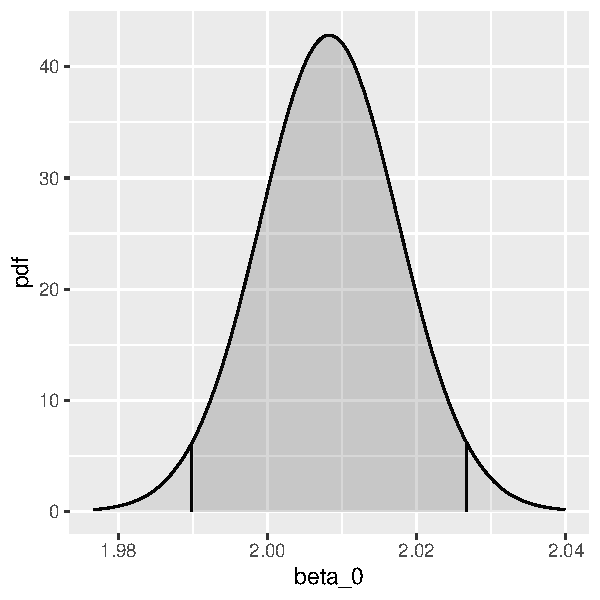
\includegraphics[keepaspectratio]{day1_practical_2_files/figure-pdf/unnamed-chunk-10-1.pdf}}
\end{center}

\begin{tcolorbox}[enhanced jigsaw, titlerule=0mm, breakable, opacitybacktitle=0.6, rightrule=.15mm, left=2mm, arc=.35mm, toptitle=1mm, coltitle=black, colframe=quarto-callout-warning-color-frame, opacityback=0, colback=white, bottomrule=.15mm, leftrule=.75mm, colbacktitle=quarto-callout-warning-color!10!white, bottomtitle=1mm, title={Task}, toprule=.15mm]

Plot the posterior marginals for \(\beta_1\) and for the precision of
the observation error \(\pi(\tau|y)\)

Take hint

See the \texttt{summary()} output to check the names for the different
model components.

Click here to see the solution

\begin{Shaded}
\begin{Highlighting}[]
\FunctionTok{plot}\NormalTok{(fit.lm, }\StringTok{"beta\_1"}\NormalTok{) }\SpecialCharTok{+}
\FunctionTok{plot}\NormalTok{(fit.lm, }\StringTok{"Precision for the Gaussian observations"}\NormalTok{)}
\end{Highlighting}
\end{Shaded}

\begin{center}
\pandocbounded{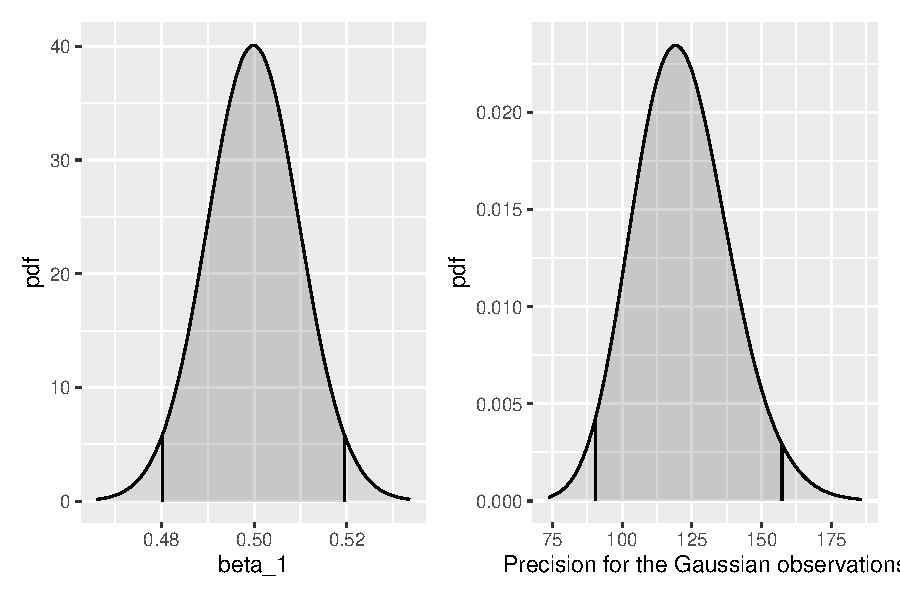
\includegraphics[keepaspectratio]{day1_practical_2_files/figure-pdf/unnamed-chunk-11-1.pdf}}
\end{center}

\end{tcolorbox}

\subsubsection{Model Checking}\label{model-checking}

A common way for model diagnostics in regression analysis is by checking
residual plots. In a Bayesian setting residuals can be defined in
multipleways depending on how you account for posterior uncertainty.
Here, we will adopt a Bayesian approach by generating samples from the
posterior distribution of the model parameters and then draw samples
from the residuals defined as:

\[
r_i = y_i - x_i^T\beta
\]

We can use the \texttt{predict} function to achieve this:

\begin{Shaded}
\begin{Highlighting}[]
\NormalTok{res\_samples }\OtherTok{\textless{}{-}} \FunctionTok{predict}\NormalTok{(}
\NormalTok{  fit.lm,         }\CommentTok{\# the fitted model}
\NormalTok{  df,             }\CommentTok{\# the original data set}
  \SpecialCharTok{\textasciitilde{}} \FunctionTok{data.frame}\NormalTok{(   }
    \AttributeTok{res =}\NormalTok{ y}\SpecialCharTok{{-}}\NormalTok{(beta\_0 }\SpecialCharTok{+}\NormalTok{ beta\_1)  }\CommentTok{\# compute the residuals}
\NormalTok{  ),}
  \AttributeTok{n.samples =} \DecValTok{1000}   \CommentTok{\# draw 1000 samples}
\NormalTok{)}
\end{Highlighting}
\end{Shaded}

The resulting data frame contains the posterior draw of the residuals
mean for which we can produce some diagnostics plots , e.g.

\begin{Shaded}
\begin{Highlighting}[]
\FunctionTok{ggplot}\NormalTok{(res\_samples,}\FunctionTok{aes}\NormalTok{(}\AttributeTok{y=}\NormalTok{mean,}\AttributeTok{x=}\DecValTok{1}\SpecialCharTok{:}\DecValTok{100}\NormalTok{))}\SpecialCharTok{+}\FunctionTok{geom\_point}\NormalTok{() }\SpecialCharTok{+}
\FunctionTok{ggplot}\NormalTok{(res\_samples,}\FunctionTok{aes}\NormalTok{(}\AttributeTok{y=}\NormalTok{mean,}\AttributeTok{x=}\NormalTok{x))}\SpecialCharTok{+}\FunctionTok{geom\_point}\NormalTok{()}
\end{Highlighting}
\end{Shaded}

\begin{figure}[H]

{\centering \pandocbounded{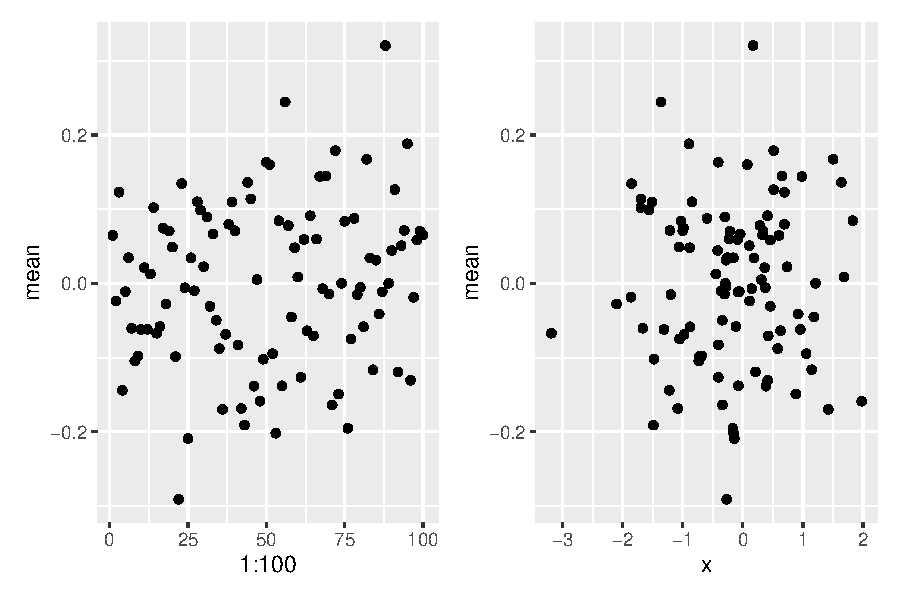
\includegraphics[keepaspectratio]{day1_practical_2_files/figure-pdf/unnamed-chunk-13-1.pdf}}

}

\caption{Bayesian residual plots: the left panel is the residual index
plot; the right panel is the plot of the residual versus the covariate
x}

\end{figure}%

We can also compare these against the theoretical quantiles of the
Normal distribution as follows:

\begin{Shaded}
\begin{Highlighting}[]
\FunctionTok{arrange}\NormalTok{(res\_samples, mean) }\SpecialCharTok{\%\textgreater{}\%}
  \FunctionTok{mutate}\NormalTok{(}\AttributeTok{theortical\_quantiles =} \FunctionTok{qnorm}\NormalTok{(}\DecValTok{1}\SpecialCharTok{:}\DecValTok{100} \SpecialCharTok{/}\NormalTok{ (}\DecValTok{1}\SpecialCharTok{+}\DecValTok{100}\NormalTok{))) }\SpecialCharTok{\%\textgreater{}\%}
  \FunctionTok{ggplot}\NormalTok{(}\FunctionTok{aes}\NormalTok{(}\AttributeTok{x=}\NormalTok{theortical\_quantiles,}\AttributeTok{y=}\NormalTok{ mean)) }\SpecialCharTok{+} 
  \FunctionTok{geom\_ribbon}\NormalTok{(}\FunctionTok{aes}\NormalTok{(}\AttributeTok{ymin =}\NormalTok{ q0}\FloatTok{.025}\NormalTok{, }\AttributeTok{ymax =}\NormalTok{ q0}\FloatTok{.975}\NormalTok{), }\AttributeTok{fill =} \StringTok{"grey70"}\NormalTok{)}\SpecialCharTok{+}
  \FunctionTok{geom\_abline}\NormalTok{(}\AttributeTok{intercept =} \FunctionTok{mean}\NormalTok{(res\_samples}\SpecialCharTok{$}\NormalTok{mean),}
              \AttributeTok{slope =} \FunctionTok{sd}\NormalTok{(res\_samples}\SpecialCharTok{$}\NormalTok{mean)) }\SpecialCharTok{+}
  \FunctionTok{geom\_point}\NormalTok{() }\SpecialCharTok{+}
  \FunctionTok{labs}\NormalTok{(}\AttributeTok{x =} \StringTok{"Theoretical Quantiles (Normal)"}\NormalTok{,}
       \AttributeTok{y=} \StringTok{"Sample Quantiles (Residuals)"}\NormalTok{) }
\end{Highlighting}
\end{Shaded}

\begin{center}
\pandocbounded{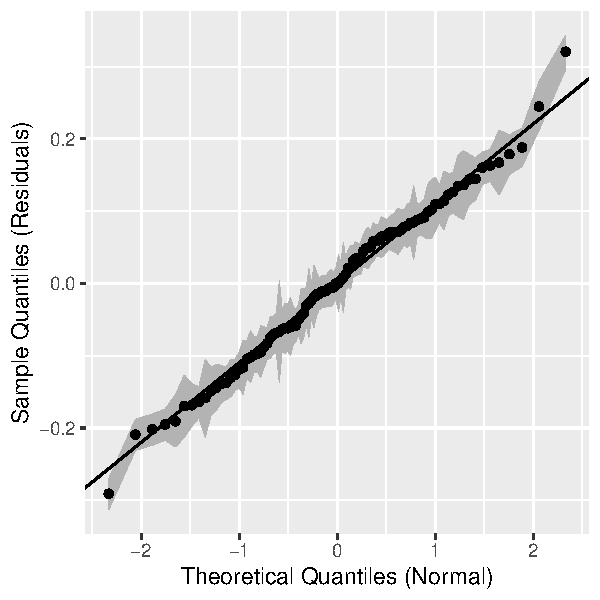
\includegraphics[keepaspectratio]{day1_practical_2_files/figure-pdf/unnamed-chunk-14-1.pdf}}
\end{center}

\subsection{Linear Mixed Model for fish weight-length
relationship}\label{sec-llm_fish}

In this exercise we will:

\begin{itemize}
\tightlist
\item
  Plot random effects of a LMM
\item
  Compute posterior densities and summaries for the variance components
\end{itemize}

Libraries to load:

\begin{Shaded}
\begin{Highlighting}[]
\FunctionTok{library}\NormalTok{(dplyr)}
\FunctionTok{library}\NormalTok{(INLA)}
\FunctionTok{library}\NormalTok{(ggplot2)}
\FunctionTok{library}\NormalTok{(patchwork)}
\FunctionTok{library}\NormalTok{(inlabru)     }
\end{Highlighting}
\end{Shaded}

In this exercise, we will use a subset of the Pygmy Whitefish
(\emph{Prosopium coulterii}) dataset from the \texttt{FSAdata} R
package, containing biological data collected in 2001 from Dina Lake,
British Columbia.

The data set contains the following information:

\begin{itemize}
\tightlist
\item
  \texttt{net\_no}Unique net identification number
\item
  \texttt{wt} Fish weight (g)
\item
  \texttt{tl} Total fish length (cm)
\item
  \texttt{sex} Sex code (\texttt{F}=Female, \texttt{M} = Male)
\end{itemize}

We can visualize the distribution of the response (weight) across the
nets split by sex as follows:

\begin{Shaded}
\begin{Highlighting}[]
\NormalTok{PygmyWFBC }\OtherTok{\textless{}{-}} \FunctionTok{read.csv}\NormalTok{(}\StringTok{"datasets/PygmyWFBC.csv"}\NormalTok{)}

\FunctionTok{ggplot}\NormalTok{(PygmyWFBC, }\FunctionTok{aes}\NormalTok{(}\AttributeTok{x =} \FunctionTok{factor}\NormalTok{(net\_no), }\AttributeTok{y =}\NormalTok{ wt,}\AttributeTok{fill =}\NormalTok{ sex)) }\SpecialCharTok{+} 
  \FunctionTok{geom\_boxplot}\NormalTok{() }\SpecialCharTok{+} 
  \FunctionTok{labs}\NormalTok{(}\AttributeTok{y=}\StringTok{"Weight (g)"}\NormalTok{,}\AttributeTok{x =} \StringTok{"Net no."}\NormalTok{)}
\end{Highlighting}
\end{Shaded}

\begin{center}
\pandocbounded{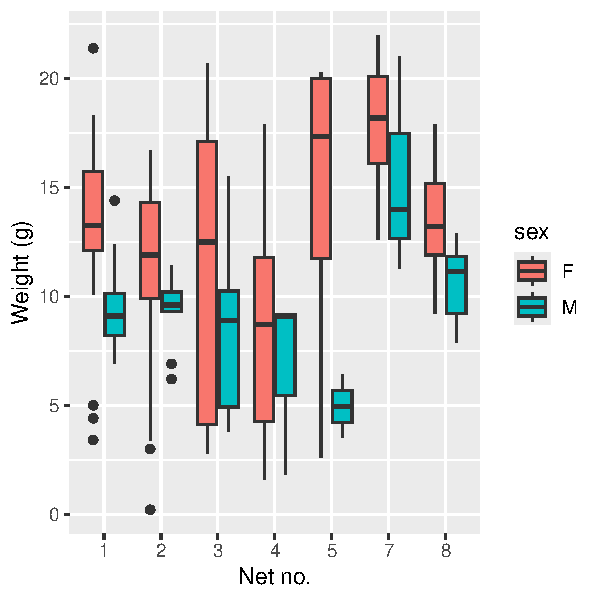
\includegraphics[keepaspectratio]{day1_practical_2_files/figure-pdf/unnamed-chunk-17-1.pdf}}
\end{center}

Suppose we are interested in modelling the weight-length relationship
for captured fish. The exploratory plot suggest some important
variability in this relationship, potentially attributable to
differences among sampling nets deployed across various sites in the
Dina Lake.

To account for this between-net variability, we model net as a random
effect using the following linear mixed model:

\[
\begin{aligned}
y_{ij} &\sim\mathcal{N}(\mu_{ij}, \sigma_e^2), \qquad i = 1,\dots,a \qquad j = 1,\ldots,n \\
\eta_{ij} &= \mu_{ij} = \beta_0 + \beta_1 \times \text{length}_j + \beta_2 \times \mathbb{I}(\mathrm{Sex}_{ij}=\mathrm{M}) +  u_i \\
u_i &\sim \mathcal{N}(0,\sigma^2_u)
\end{aligned}
\]

where:

\begin{itemize}
\item
  \(y_{ij}\) is the weight of the \(j\)-th fish from net \(i\)
\item
  \(\text{length}_{ij}\) is the corresponding fish length
\item
  \(\mathbb{I}(\text{Sex}_{ij} = \text{M})\) is an indicator/dummy such
  that for the \emph{i}th net \[
  \mathbb{I}(\mathrm{Sex}_{ij}) \begin{cases}1 & \text{if the } j \text{th fish is Male} \\0 & \text{otherwise} \end{cases}
  \]
\item
  \(u_i\) represents the random intercept for net \(i\)
\item
  \(\sigma_u^2\) and \(\sigma_\epsilon^2\) are the between-net and
  residual variances, respectively
\end{itemize}

To run this model in\texttt{inlabru} we first need to create our sex
dummy variable :

\begin{Shaded}
\begin{Highlighting}[]
\NormalTok{PygmyWFBC}\SpecialCharTok{$}\NormalTok{sex\_M }\OtherTok{\textless{}{-}} \FunctionTok{ifelse}\NormalTok{(PygmyWFBC}\SpecialCharTok{$}\NormalTok{sex}\SpecialCharTok{==}\StringTok{"F"}\NormalTok{,}\DecValTok{0}\NormalTok{,}\DecValTok{1}\NormalTok{)}
\end{Highlighting}
\end{Shaded}

\texttt{inlabru} will treat 0 as the reference category (i.e., the
intercept \(\beta_0\) will represent the baseline weight for females ).
Now we can define the model component, the likelihood and fit the model.

\begin{Shaded}
\begin{Highlighting}[]
\NormalTok{cmp }\OtherTok{=}  \ErrorTok{\textasciitilde{}} \SpecialCharTok{{-}}\DecValTok{1} \SpecialCharTok{+}\NormalTok{ sex\_M }\SpecialCharTok{+}  \FunctionTok{beta\_0}\NormalTok{(}\DecValTok{1}\NormalTok{)  }\SpecialCharTok{+} \FunctionTok{beta\_1}\NormalTok{(tl, }\AttributeTok{model =} \StringTok{"linear"}\NormalTok{) }\SpecialCharTok{+}   \FunctionTok{net\_eff}\NormalTok{(net\_no, }\AttributeTok{model =} \StringTok{"iid"}\NormalTok{)}

\NormalTok{lik }\OtherTok{=}  \FunctionTok{bru\_obs}\NormalTok{(}\AttributeTok{formula =}\NormalTok{ wt }\SpecialCharTok{\textasciitilde{}}\NormalTok{ .,}
            \AttributeTok{family =} \StringTok{"gaussian"}\NormalTok{,}
            \AttributeTok{data =}\NormalTok{ PygmyWFBC)}

\NormalTok{fit }\OtherTok{=} \FunctionTok{bru}\NormalTok{(cmp, lik)}

\FunctionTok{summary}\NormalTok{(fit)}
\end{Highlighting}
\end{Shaded}

\begin{verbatim}
inlabru version: 2.13.0
INLA version: 25.08.21-1
Components:
sex_M: main = linear(sex_M), group = exchangeable(1L), replicate = iid(1L), NULL
beta_0: main = linear(1), group = exchangeable(1L), replicate = iid(1L), NULL
beta_1: main = linear(tl), group = exchangeable(1L), replicate = iid(1L), NULL
net_eff: main = iid(net_no), group = exchangeable(1L), replicate = iid(1L), NULL
Observation models:
  Family: 'gaussian'
    Tag: <No tag>
    Data class: 'data.frame'
    Response class: 'numeric'
    Predictor: wt ~ .
    Additive/Linear: TRUE/TRUE
    Used components: effects[sex_M, beta_0, beta_1, net_eff], latent[]
Time used:
    Pre = 0.306, Running = 0.303, Post = 0.141, Total = 0.75 
Fixed effects:
          mean    sd 0.025quant 0.5quant 0.975quant    mode kld
sex_M   -1.106 0.218     -1.534   -1.106     -0.678  -1.106   0
beta_0 -15.816 0.870    -17.515  -15.819    -14.100 -15.819   0
beta_1   2.555 0.072      2.414    2.555      2.696   2.555   0

Random effects:
  Name    Model
    net_eff IID model

Model hyperparameters:
                                         mean    sd 0.025quant 0.5quant
Precision for the Gaussian observations 0.475 0.044      0.392    0.473
Precision for net_eff                   2.151 1.331      0.558    1.837
                                        0.975quant mode
Precision for the Gaussian observations      0.567 0.47
Precision for net_eff                        5.581 1.31

Marginal log-Likelihood:  -467.53 
 is computed 
Posterior summaries for the linear predictor and the fitted values are computed
(Posterior marginals needs also 'control.compute=list(return.marginals.predictor=TRUE)')
\end{verbatim}

For interpretability, we could have centered the predictors, but our
primary focus here is on estimating the variance components of the mixed
model.

We can plot the posterior density of the nets random intercept as
follows:

\begin{Shaded}
\begin{Highlighting}[]
\FunctionTok{plot}\NormalTok{(fit,}\StringTok{"net\_eff"}\NormalTok{)}
\end{Highlighting}
\end{Shaded}

\pandocbounded{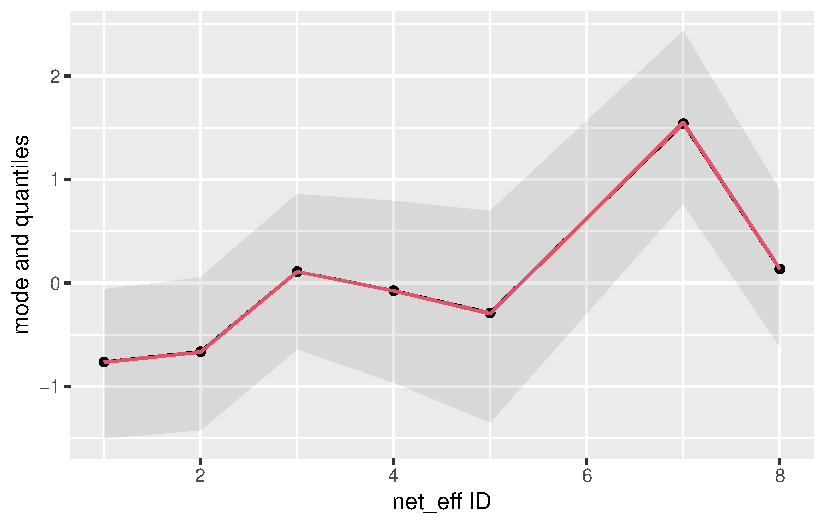
\includegraphics[keepaspectratio]{day1_practical_2_files/figure-pdf/unnamed-chunk-20-1.pdf}}

For theoretical and computational purposes, INLA works with the
precision which is the inverse of the variance. To obtain the posterior
summaries on the SDs scale we can sample from the posterior distribution
for the precision while back-transforming the samples and then computing
the summary statistics. Transforming the samples is necessary because
some quantities such as the mean and mode are not invariant to monotone
transformation; alternatively we can use some of the in-built
\texttt{R-INLA} functions to achieve this (see supplementary note).

We use the \texttt{inla.hyperpar.sample} function to draw samples from
the approximated joint posterior for the hyperparameters, then invert
them to get variances and lastly compute the mean, std. dev., quantiles,
etc.

\begin{Shaded}
\begin{Highlighting}[]
\NormalTok{sampvars }\OtherTok{\textless{}{-}} \DecValTok{1}\SpecialCharTok{/}\FunctionTok{inla.hyperpar.sample}\NormalTok{(}\DecValTok{1000}\NormalTok{,fit,}\AttributeTok{improve.marginals =}\NormalTok{ T)}

\FunctionTok{colnames}\NormalTok{(sampvars) }\OtherTok{\textless{}{-}} \FunctionTok{c}\NormalTok{(}\StringTok{"Error variance"}\NormalTok{,}\StringTok{"Between{-}net Variance"}\NormalTok{)}

\FunctionTok{apply}\NormalTok{(sampvars,}\DecValTok{2}\NormalTok{,}
      \ControlFlowTok{function}\NormalTok{(x) }\FunctionTok{c}\NormalTok{(}\StringTok{"mean"}\OtherTok{=}\FunctionTok{mean}\NormalTok{(x),}
                    \StringTok{"std.dev"} \OtherTok{=} \FunctionTok{sd}\NormalTok{(x),}
                    \FunctionTok{quantile}\NormalTok{(x,}\FunctionTok{c}\NormalTok{(}\FloatTok{0.025}\NormalTok{,}\FloatTok{0.5}\NormalTok{,}\FloatTok{0.975}\NormalTok{))))}
\end{Highlighting}
\end{Shaded}

\begin{verbatim}
        Error variance Between-net Variance
mean         2.1253048            0.6533978
std.dev      0.1983667            0.4209485
2.5%         1.7684930            0.1818261
50%          2.1140833            0.5436095
97.5%        2.5434788            1.7644842
\end{verbatim}

\begin{tcolorbox}[enhanced jigsaw, titlerule=0mm, breakable, opacitybacktitle=0.6, rightrule=.15mm, left=2mm, arc=.35mm, toptitle=1mm, coltitle=black, colframe=quarto-callout-warning-color-frame, opacityback=0, colback=white, bottomrule=.15mm, leftrule=.75mm, colbacktitle=quarto-callout-warning-color!10!white, bottomtitle=1mm, title={Task}, toprule=.15mm]

Another useful quantity we can compute is the intraclass correlation
coefficient (ICC) which help us determine how much the response varies
within groups compared to between groups. The intraclass correlation
coefficient is defined as:

\[
\text{ICC} = \frac{\sigma^2_u}{\sigma^2_u + \sigma^2_e}
\]

Compute the median, and quantiles for the ICC using the posterior
samples we draw for \(\sigma^2_e\) and \(\sigma^2_u\).

Take hint

The \texttt{rowSums} function can be used to compute
\(\sigma^2_{u,s} + \sigma^2_{e,s}\) for the \(s\)th posterior draw.

Click here to see the solution

\begin{Shaded}
\begin{Highlighting}[]
\NormalTok{sampicc }\OtherTok{\textless{}{-}}\NormalTok{ sampvars[,}\DecValTok{2}\NormalTok{]}\SpecialCharTok{/}\NormalTok{(}\FunctionTok{rowSums}\NormalTok{(sampvars))}
\FunctionTok{quantile}\NormalTok{(sampicc, }\FunctionTok{c}\NormalTok{(}\FloatTok{0.025}\NormalTok{,}\FloatTok{0.5}\NormalTok{,}\FloatTok{0.975}\NormalTok{))}
\end{Highlighting}
\end{Shaded}

\begin{verbatim}
      2.5%        50%      97.5% 
0.07766672 0.20463154 0.46566811 
\end{verbatim}

\end{tcolorbox}

\begin{tcolorbox}[enhanced jigsaw, titlerule=0mm, breakable, opacitybacktitle=0.6, rightrule=.15mm, left=2mm, arc=.35mm, toptitle=1mm, coltitle=black, colframe=quarto-callout-note-color-frame, opacityback=0, colback=white, bottomrule=.15mm, leftrule=.75mm, colbacktitle=quarto-callout-note-color!10!white, bottomtitle=1mm, title=\textcolor{quarto-callout-note-color}{\faInfo}\hspace{0.5em}{Supplementary Material}, toprule=.15mm]

The marginal densities for the hyper parameters can be also found by
calling\texttt{inlabru\_model\$marginals.hyperpar}. We can then apply a
transformation using the \texttt{inla.tmarginal} function to transform
the precision posterior distributions.

\begin{Shaded}
\begin{Highlighting}[]
\NormalTok{var\_e }\OtherTok{\textless{}{-}}\NormalTok{ fit}\SpecialCharTok{$}\NormalTok{marginals.hyperpar}\SpecialCharTok{$}\StringTok{\textasciigrave{}}\AttributeTok{Precision for the Gaussian observations}\StringTok{\textasciigrave{}} \SpecialCharTok{\%\textgreater{}\%}
  \FunctionTok{inla.tmarginal}\NormalTok{(}\ControlFlowTok{function}\NormalTok{(x) }\DecValTok{1}\SpecialCharTok{/}\NormalTok{x,.) }

\NormalTok{var\_u }\OtherTok{\textless{}{-}}\NormalTok{ fit}\SpecialCharTok{$}\NormalTok{marginals.hyperpar}\SpecialCharTok{$}\StringTok{\textasciigrave{}}\AttributeTok{Precision for net\_eff}\StringTok{\textasciigrave{}} \SpecialCharTok{\%\textgreater{}\%}
  \FunctionTok{inla.tmarginal}\NormalTok{(}\ControlFlowTok{function}\NormalTok{(x) }\DecValTok{1}\SpecialCharTok{/}\NormalTok{x,.) }
\end{Highlighting}
\end{Shaded}

The marginal densities for the hyper parameters can be found with
\texttt{inlabru\_model\$marginals.hyperpar}, then we can apply a
transformation using the \texttt{inla.tmarginal} function to transform
the precision posterior distributions. Then, we can compute posterior
summaries using \texttt{inla.zmarginal} function as follows:

\begin{Shaded}
\begin{Highlighting}[]
\NormalTok{post\_var\_summaries }\OtherTok{\textless{}{-}} \FunctionTok{cbind}\NormalTok{( }\FunctionTok{inla.zmarginal}\NormalTok{(var\_e,}\AttributeTok{silent =}\NormalTok{ T),}
                             \FunctionTok{inla.zmarginal}\NormalTok{(var\_u,}\AttributeTok{silent =}\NormalTok{ T))}
\FunctionTok{colnames}\NormalTok{(post\_var\_summaries) }\OtherTok{\textless{}{-}} \FunctionTok{c}\NormalTok{(}\StringTok{"sigma\_e"}\NormalTok{,}\StringTok{"sigma\_u"}\NormalTok{)}
\NormalTok{post\_var\_summaries}
\end{Highlighting}
\end{Shaded}

\begin{verbatim}
           sigma_e  sigma_u  
mean       2.124886 0.6527294
sd         0.198279 0.4212976
quant0.025 1.7665   0.1796571
quant0.25  1.985474 0.3677913
quant0.5   2.11334  0.5419084
quant0.75  2.252102 0.8103722
quant0.975 2.54464  1.77092  
\end{verbatim}

\end{tcolorbox}

\subsection{GLM model checking}\label{sec-linmodel}

In this exercise we will:

\begin{itemize}
\tightlist
\item
  Learn about some model assessments techniques available in INLA
\item
  Conduct posterior predictive model checking
\end{itemize}

Libraries to load:

\begin{Shaded}
\begin{Highlighting}[]
\FunctionTok{library}\NormalTok{(dplyr)}
\FunctionTok{library}\NormalTok{(INLA)}
\FunctionTok{library}\NormalTok{(ggplot2)}
\FunctionTok{library}\NormalTok{(patchwork)}
\FunctionTok{library}\NormalTok{(inlabru)     }
\end{Highlighting}
\end{Shaded}

In this exercise, we will use data on horseshoe crabs (\emph{Limulus
polyphemus}) where the number of satellites males surrounding a breeding
female are counted along with the female's color and carapace width.

A possible model to study the factors that affect the number of
satellites for female crabs is

\[
\begin{aligned}
y_i&\sim\mathrm{Poisson}(\mu_i), \qquad i = 1,\dots,N \\
\eta_i &= \mu_i = \beta_0 + \beta_1 x_i + \ldots
\end{aligned}
\]

We can explore the conditional means and variances given the female's
color:

\begin{Shaded}
\begin{Highlighting}[]
\NormalTok{crabs }\OtherTok{\textless{}{-}} \FunctionTok{read.csv}\NormalTok{(}\StringTok{"datasets/crabs.csv"}\NormalTok{)}

\CommentTok{\# conditional means and variances}
\NormalTok{crabs }\SpecialCharTok{\%\textgreater{}\%}
  \FunctionTok{summarise}\NormalTok{( }\AttributeTok{Mean =} \FunctionTok{mean}\NormalTok{(satell ),}
             \AttributeTok{Variance =} \FunctionTok{var}\NormalTok{(satell),}
                     \AttributeTok{.by =}\NormalTok{ color)}
\end{Highlighting}
\end{Shaded}

\begin{verbatim}
   color     Mean  Variance
1 medium 3.294737 10.273908
2   dark 2.227273  6.737844
3  light 4.083333  9.719697
4 darker 2.045455 13.093074
\end{verbatim}

The mean of the number of satellites vary by color which gives a good
indication that color might be useful for predicting satellites numbers.
However, notice that the mean is lower than its variance suggesting that
overdispersion might be present and that a negative binomial model would
be more appropriate for the data (we will cover this later).

\textbf{Fitting the model}

First, lets begin fitting the Poisson model above using the carapace's
color and width as predictors. Since, color is a categorical variable in
our model we need to create a dummy variable for it. We can use the
\texttt{model.matrix} function to help us constructing the design matrix
and then append this to our data:

\begin{Shaded}
\begin{Highlighting}[]
\NormalTok{crabs\_df }\OtherTok{=} \FunctionTok{model.matrix}\NormalTok{( }\SpecialCharTok{\textasciitilde{}}\NormalTok{  color , crabs) }\SpecialCharTok{\%\textgreater{}\%}
  \FunctionTok{as.data.frame}\NormalTok{() }\SpecialCharTok{\%\textgreater{}\%}
  \FunctionTok{select}\NormalTok{(}\SpecialCharTok{{-}}\DecValTok{1}\NormalTok{) }\SpecialCharTok{\%\textgreater{}\%}        \CommentTok{\# drop intercept}
  \FunctionTok{bind\_cols}\NormalTok{(crabs) }\SpecialCharTok{\%\textgreater{}\%}  \CommentTok{\# append to original data}
  \FunctionTok{select}\NormalTok{(}\SpecialCharTok{{-}}\NormalTok{color)        }\CommentTok{\# remove original color categorical variable}
\end{Highlighting}
\end{Shaded}

The new data set \texttt{crabs\_df} contains a dummy variable for the
different color categories (\texttt{dark} being the reference category).
Then we can fit the model in \texttt{inlabru} as follows:

\begin{Shaded}
\begin{Highlighting}[]
\NormalTok{cmp }\OtherTok{=}  \ErrorTok{\textasciitilde{}} \SpecialCharTok{{-}}\DecValTok{1} \SpecialCharTok{+} \FunctionTok{beta0}\NormalTok{(}\DecValTok{1}\NormalTok{) }\SpecialCharTok{+}\NormalTok{  colordarker }\SpecialCharTok{+}
\NormalTok{       colorlight }\SpecialCharTok{+}\NormalTok{ colormedium }\SpecialCharTok{+}
       \FunctionTok{w}\NormalTok{(weight, }\AttributeTok{model =} \StringTok{"linear"}\NormalTok{)}

\NormalTok{lik }\OtherTok{=}  \FunctionTok{bru\_obs}\NormalTok{(}\AttributeTok{formula =}\NormalTok{ satell }\SpecialCharTok{\textasciitilde{}}\NormalTok{.,}
            \AttributeTok{family =} \StringTok{"poisson"}\NormalTok{,}
            \AttributeTok{data =}\NormalTok{ crabs\_df)}

\NormalTok{fit\_pois }\OtherTok{=} \FunctionTok{bru}\NormalTok{(cmp, lik)}

\FunctionTok{summary}\NormalTok{(fit\_pois)}
\end{Highlighting}
\end{Shaded}

\begin{verbatim}
inlabru version: 2.13.0
INLA version: 25.08.21-1
Components:
beta0: main = linear(1), group = exchangeable(1L), replicate = iid(1L), NULL
colordarker: main = linear(colordarker), group = exchangeable(1L), replicate = iid(1L), NULL
colorlight: main = linear(colorlight), group = exchangeable(1L), replicate = iid(1L), NULL
colormedium: main = linear(colormedium), group = exchangeable(1L), replicate = iid(1L), NULL
w: main = linear(weight), group = exchangeable(1L), replicate = iid(1L), NULL
Observation models:
  Family: 'poisson'
    Tag: <No tag>
    Data class: 'data.frame'
    Response class: 'integer'
    Predictor: satell ~ .
    Additive/Linear: TRUE/TRUE
    Used components: effects[beta0, colordarker, colorlight, colormedium, w], latent[]
Time used:
    Pre = 0.292, Running = 0.246, Post = 0.0555, Total = 0.593 
Fixed effects:
              mean    sd 0.025quant 0.5quant 0.975quant   mode kld
beta0       -0.501 0.196     -0.885   -0.501     -0.117 -0.501   0
colordarker -0.008 0.180     -0.362   -0.008      0.345 -0.008   0
colorlight   0.445 0.176      0.101    0.445      0.790  0.445   0
colormedium  0.248 0.118      0.017    0.248      0.479  0.248   0
w            0.001 0.000      0.000    0.001      0.001  0.001   0

Marginal log-Likelihood:  -489.43 
 is computed 
Posterior summaries for the linear predictor and the fitted values are computed
(Posterior marginals needs also 'control.compute=list(return.marginals.predictor=TRUE)')
\end{verbatim}

\subsubsection{Model assessment and model
choice}\label{model-assessment-and-model-choice}

Now that we have fitted the model we would like to carry some model
assessments. In a Bayesian setting, this is often based on posterior
predictive checks. To do so, we will use the CPO and PIT - two commonly
used Bayesian model assessment criteria based on the \textbf{posterior
predictive distribution}.

\begin{tcolorbox}[enhanced jigsaw, titlerule=0mm, breakable, opacitybacktitle=0.6, rightrule=.15mm, left=2mm, arc=.35mm, toptitle=1mm, coltitle=black, colframe=quarto-callout-note-color-frame, opacityback=0, colback=white, bottomrule=.15mm, leftrule=.75mm, colbacktitle=quarto-callout-note-color!10!white, bottomtitle=1mm, title=\textcolor{quarto-callout-note-color}{\faInfo}\hspace{0.5em}{Posterior predictive model checking}, toprule=.15mm]

The posterior predictive distribution for a predicted value \(\hat{y}\)
is

\[
\pi(\hat{y}|\mathbf{y}) = \int_\theta \pi(\hat{y}|\theta)\pi(\theta|\mathbf{y})d\theta.
\]

The probability integral transform (PIT) introduced by Dawid (1984) is
defined for each observation as:

\[
\mathrm{PIT}_i = \pi(\hat{y}_i \leq y_i |\mathbf{y}{-i})
\]

The PIT evaluates how well a model's predicted values match the observed
data distribution. It is computed as the cumulative distribution
function (CDF) of the observed data evaluated at each predicted value.
If the model is well-calibrated, the PIT values should be
\emph{approximately uniformly distributed}. Deviations from this uniform
distribution may indicate issues with model calibration or overfitting.

Another metric we could used to asses the model fit is the conditional
predictive ordinate (CPO) introduced by Pettit (1990), and defined as:

\[
\text{CPO}_i = \pi(y_i| \mathbf{y}{-i})
\]

The CPO measures the probability of the observed value of \(y_i\) when
model is fit using all data but \(y_i\). CPO provides a measure of how
well the model predicts each individual observation while taking into
account the rest of the data and the model. \emph{Large values indicate
a better fit} of the model to the data, while small values indicate a
bad fitting of the model

\end{tcolorbox}

To compute PIT and CPO we can either:

\begin{enumerate}
\def\labelenumi{\arabic{enumi}.}
\item
  ask \texttt{inlabru} to compute them by set
  \texttt{options\ =\ list(control.compute\ =\ list(cpo\ =\ TRUE))} in
  the \texttt{bru()} function arguments.
\item
  set this as default in \texttt{inlabru} global option using the
  \texttt{bru\_options\_set} function.
\end{enumerate}

Here we will do the later and re-run the model

\begin{Shaded}
\begin{Highlighting}[]
\FunctionTok{bru\_options\_set}\NormalTok{(}\AttributeTok{control.compute =} \FunctionTok{list}\NormalTok{(}\AttributeTok{cpo =} \ConstantTok{TRUE}\NormalTok{))}

\NormalTok{fit\_pois }\OtherTok{=} \FunctionTok{bru}\NormalTok{(cmp, lik)}
\end{Highlighting}
\end{Shaded}

Now we can produce histograms and QQ plots to assess for uniformity in
the PIT values which can be accessed through
\texttt{inlabru\_model\$cpo\$pit} :

\section{Plot}

\begin{center}
\pandocbounded{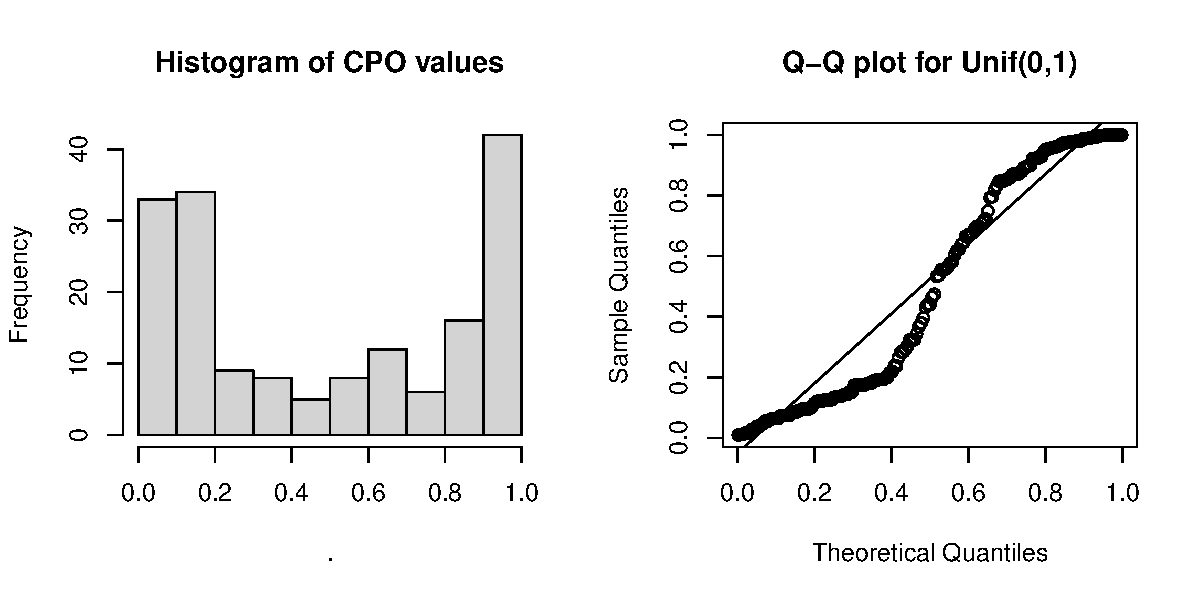
\includegraphics[keepaspectratio]{day1_practical_2_files/figure-pdf/unnamed-chunk-32-1.pdf}}
\end{center}

\section{R Code}

\begin{Shaded}
\begin{Highlighting}[]
\NormalTok{fit\_pois}\SpecialCharTok{$}\NormalTok{cpo}\SpecialCharTok{$}\NormalTok{pit }\SpecialCharTok{\%\textgreater{}\%}
  \FunctionTok{hist}\NormalTok{(}\AttributeTok{main =} \StringTok{"Histogram of PIT values"}\NormalTok{)}

\FunctionTok{qqplot}\NormalTok{(}\FunctionTok{qunif}\NormalTok{(}\FunctionTok{ppoints}\NormalTok{(}\FunctionTok{length}\NormalTok{(fit\_pois}\SpecialCharTok{$}\NormalTok{cpo}\SpecialCharTok{$}\NormalTok{pit))),}
\NormalTok{       fit\_pois}\SpecialCharTok{$}\NormalTok{cpo}\SpecialCharTok{$}\NormalTok{pit,}
       \AttributeTok{main =} \StringTok{"Q{-}Q plot for Unif(0,1)"}\NormalTok{,}
       \AttributeTok{xlab =} \StringTok{"Theoretical Quantiles"}\NormalTok{,}
       \AttributeTok{ylab =} \StringTok{"Sample Quantiles"}\NormalTok{)}

\FunctionTok{qqline}\NormalTok{(fit\_pois}\SpecialCharTok{$}\NormalTok{cpo}\SpecialCharTok{$}\NormalTok{pit,}
       \AttributeTok{distribution =} \ControlFlowTok{function}\NormalTok{(p) }\FunctionTok{qunif}\NormalTok{(p),}
       \AttributeTok{prob =} \FunctionTok{c}\NormalTok{(}\FloatTok{0.1}\NormalTok{, }\FloatTok{0.9}\NormalTok{))}
\end{Highlighting}
\end{Shaded}

Both Q-Q plots and histogram of the PIT values suggest a not so great
model fit. For the CPO values, usually the following summary of the CPO
is often used:

\[
-\sum_{i=1}^n \log (\text{CPO}\_i)
\]

This quantities is useful when comparing different models - a smaller
values indicate a better model fit. CPO values can be accessed by typing
\texttt{inlabru\_model\$cpo\$cpo}.

\begin{tcolorbox}[enhanced jigsaw, titlerule=0mm, breakable, opacitybacktitle=0.6, rightrule=.15mm, left=2mm, arc=.35mm, toptitle=1mm, coltitle=black, colframe=quarto-callout-warning-color-frame, opacityback=0, colback=white, bottomrule=.15mm, leftrule=.75mm, colbacktitle=quarto-callout-warning-color!10!white, bottomtitle=1mm, title={Task}, toprule=.15mm]

The model assessment above suggests that a Poisson model might not be
the most appropriate model, likely due to the overdispersion we detected
previously. Fit a Negative binomial to relax the Poisson model
assumption that the conditional mean and variance are equal. Then,
compute the CPO summary statistic and PIT QQ plot to decide which model
gives the better fit.

Take hint

To specify a negative binomial model you only need to change the family
distribution to \texttt{family\ =\ \ "nbinomial"}.

Click here to see the solution

\begin{Shaded}
\begin{Highlighting}[]
\FunctionTok{par}\NormalTok{(}\AttributeTok{mfrow=}\FunctionTok{c}\NormalTok{(}\DecValTok{1}\NormalTok{,}\DecValTok{2}\NormalTok{))}

\CommentTok{\# Fit the negative binomial model}

\NormalTok{lik\_nbinom }\OtherTok{=}  \FunctionTok{bru\_obs}\NormalTok{(}\AttributeTok{formula =}\NormalTok{ satell }\SpecialCharTok{\textasciitilde{}}\NormalTok{.,}
            \AttributeTok{family =} \StringTok{"nbinomial"}\NormalTok{,}
            \AttributeTok{data =}\NormalTok{ crabs\_df)}

\NormalTok{fit\_nbinom }\OtherTok{=} \FunctionTok{bru}\NormalTok{(cmp, lik\_nbinom)}

\CommentTok{\# PIT checks}

\NormalTok{fit\_nbinom}\SpecialCharTok{$}\NormalTok{cpo}\SpecialCharTok{$}\NormalTok{pit }\SpecialCharTok{\%\textgreater{}\%}
  \FunctionTok{hist}\NormalTok{(}\AttributeTok{main =} \StringTok{"Histogram of PIT values"}\NormalTok{)}

\FunctionTok{qqplot}\NormalTok{(}\FunctionTok{qunif}\NormalTok{(}\FunctionTok{ppoints}\NormalTok{(}\FunctionTok{length}\NormalTok{(fit\_nbinom}\SpecialCharTok{$}\NormalTok{cpo}\SpecialCharTok{$}\NormalTok{pit))),}
\NormalTok{       fit\_nbinom}\SpecialCharTok{$}\NormalTok{cpo}\SpecialCharTok{$}\NormalTok{pit,}
       \AttributeTok{main =} \StringTok{"Q{-}Q plot for Unif(0,1)"}\NormalTok{,}
       \AttributeTok{xlab =} \StringTok{"Theoretical Quantiles"}\NormalTok{,}
       \AttributeTok{ylab =} \StringTok{"Sample Quantiles"}\NormalTok{)}

\FunctionTok{qqline}\NormalTok{(fit\_nbinom}\SpecialCharTok{$}\NormalTok{cpo}\SpecialCharTok{$}\NormalTok{pit,}
       \AttributeTok{distribution =} \ControlFlowTok{function}\NormalTok{(p) }\FunctionTok{qunif}\NormalTok{(p),}
       \AttributeTok{prob =} \FunctionTok{c}\NormalTok{(}\FloatTok{0.1}\NormalTok{, }\FloatTok{0.9}\NormalTok{))}
\end{Highlighting}
\end{Shaded}

\begin{center}
\pandocbounded{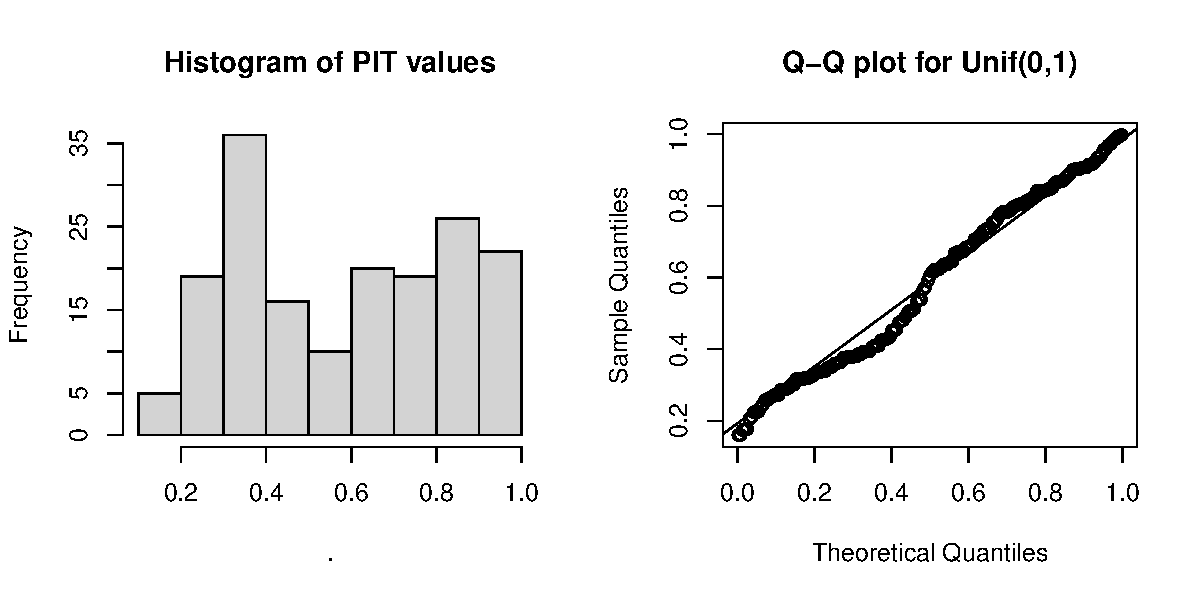
\includegraphics[keepaspectratio]{day1_practical_2_files/figure-pdf/unnamed-chunk-34-1.pdf}}
\end{center}

\begin{Shaded}
\begin{Highlighting}[]
\CommentTok{\# CPO comparison}

\FunctionTok{data.frame}\NormalTok{( }\AttributeTok{CPO =} \FunctionTok{c}\NormalTok{(}\SpecialCharTok{{-}}\FunctionTok{sum}\NormalTok{(}\FunctionTok{log}\NormalTok{(fit\_pois}\SpecialCharTok{$}\NormalTok{cpo}\SpecialCharTok{$}\NormalTok{cpo)),}
                    \SpecialCharTok{{-}}\FunctionTok{sum}\NormalTok{(}\FunctionTok{log}\NormalTok{(fit\_nbinom}\SpecialCharTok{$}\NormalTok{cpo}\SpecialCharTok{$}\NormalTok{cpo))),}
          \AttributeTok{Model =} \FunctionTok{c}\NormalTok{(}\StringTok{"Poisson"}\NormalTok{,}\StringTok{"Negative Binomial"}\NormalTok{))}
\end{Highlighting}
\end{Shaded}

\begin{verbatim}
       CPO             Model
1 465.4061           Poisson
2 379.3340 Negative Binomial
\end{verbatim}

\begin{Shaded}
\begin{Highlighting}[]
\CommentTok{\# Overall, we can see that the negative binomial model provides a better fit to the data.}
\end{Highlighting}
\end{Shaded}

\end{tcolorbox}

\subsection{\texorpdfstring{Hierarchical generalised additive mixed
models with
\texttt{inlabru}}{Hierarchical generalised additive mixed models with inlabru}}\label{hierarchical-generalised-additive-mixed-models-with-inlabru}

In this excercise we will:

\begin{itemize}
\tightlist
\item
  Fit an hierarchical generalised additive mixed models
\item
  Fit a model with a global smooth term
\item
  Fit a model with global and group-level smooth terms
\end{itemize}

Libraries to load:

\begin{Shaded}
\begin{Highlighting}[]
\FunctionTok{library}\NormalTok{(dplyr)}
\FunctionTok{library}\NormalTok{(INLA)}
\FunctionTok{library}\NormalTok{(ggplot2)}
\FunctionTok{library}\NormalTok{(patchwork)}
\FunctionTok{library}\NormalTok{(inlabru)     }
\end{Highlighting}
\end{Shaded}

The oceans represent Earth's largest habitat, with life distributed
unevenly across depths primarily due to variations in light,
temperature, and pressure. Biomass generally decreases with depth,
though complex factors like water density layers create non-linear
patterns. A significant portion of deep-sea organisms exhibit
bioluminescence, which scientists measure using specialized equipment
like free-fall camera systems to profile vertical distribution.

In this exercise, we analyze the \texttt{ISIT} dataset, which contains
bioluminescence measurements from the northeast Atlantic Ocean. This
dataset was previously examined in Zuur et
al.~(\href{https://doi.org/10.1007/978-0-387-87458-6}{2009}) and
Gillibrand et al.~(\href{https://doi.org/10.3354/meps341037}{2007}) and
consists of observations collected across a depth gradient (0--4,800 m)
during spring and summer cruises in 2001--2002 using an ISIT free-fall
profiler.

The focus of this excersice will be on characterizing seasonal variation
in the relationship between bioluminescent source density (sources
m\(^{2}\)) and depth. We begin by exploring distribution patterns of
pelagic bioluminescence through source-depth profiles, with each profile
representing measurements from an individual sampling station. These
profiles will be grouped by month to examine temporal patterns in the
water column's bioluminescent structure.

\section{Plot}

\begin{figure}[H]

{\centering \pandocbounded{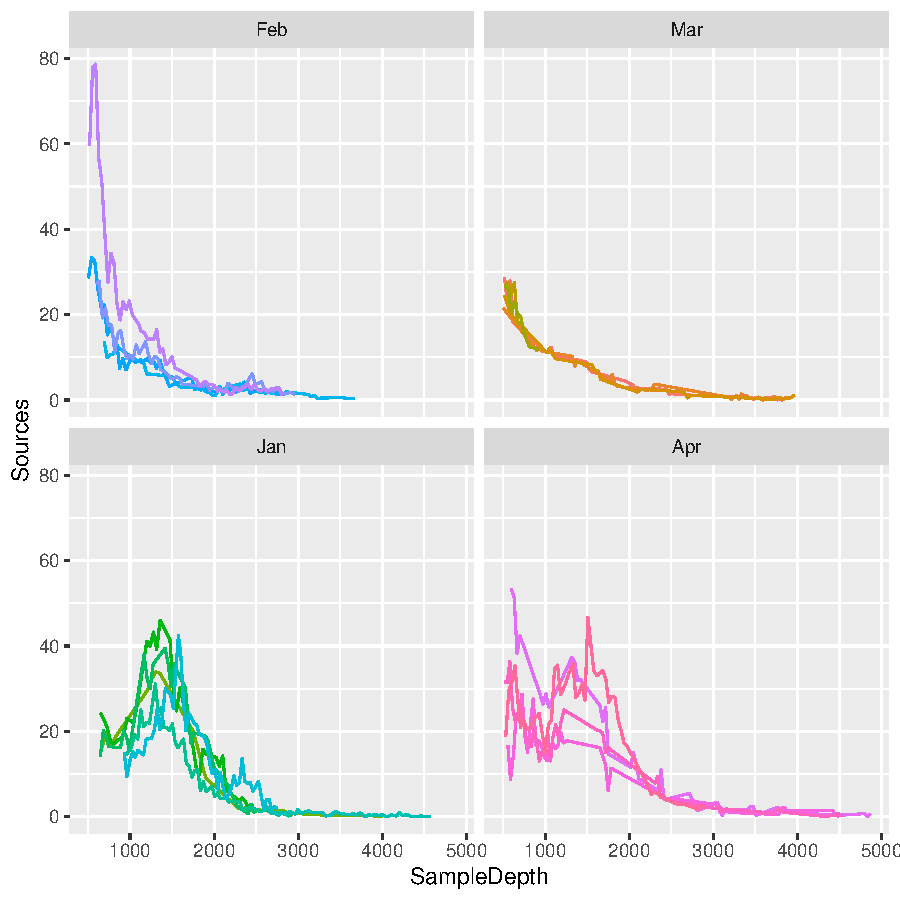
\includegraphics[keepaspectratio]{day1_practical_2_files/figure-pdf/unnamed-chunk-37-1.pdf}}

}

\caption{Source--depth profiles per month. Each line represents a
station.}

\end{figure}%

\section{R-Code}

\begin{Shaded}
\begin{Highlighting}[]
\NormalTok{icit }\OtherTok{\textless{}{-}} \FunctionTok{read.csv}\NormalTok{(}\StringTok{"datasets/ISIT.csv"}\NormalTok{)}

\NormalTok{icit}\SpecialCharTok{$}\NormalTok{Month }\OtherTok{\textless{}{-}} \FunctionTok{as.factor}\NormalTok{(icit}\SpecialCharTok{$}\NormalTok{Month)}
\FunctionTok{levels}\NormalTok{(icit}\SpecialCharTok{$}\NormalTok{Month) }\OtherTok{\textless{}{-}}\NormalTok{ month.abb[}\FunctionTok{unique}\NormalTok{(icit}\SpecialCharTok{$}\NormalTok{Month)]}

\FunctionTok{ggplot}\NormalTok{(icit,}\FunctionTok{aes}\NormalTok{(}\AttributeTok{x=}\NormalTok{SampleDepth,}\AttributeTok{y=}\NormalTok{ Sources,}
                \AttributeTok{group=}\FunctionTok{as.factor}\NormalTok{(Station),}
                \AttributeTok{colour=}\FunctionTok{as.factor}\NormalTok{(Station)))}\SpecialCharTok{+}
  \FunctionTok{geom\_line}\NormalTok{()}\SpecialCharTok{+}
  \FunctionTok{facet\_wrap}\NormalTok{(}\SpecialCharTok{\textasciitilde{}}\NormalTok{Month)}\SpecialCharTok{+}
  \FunctionTok{theme}\NormalTok{(}\AttributeTok{legend.position =} \StringTok{"none"}\NormalTok{)}
\end{Highlighting}
\end{Shaded}

As expected, there seems to be a non-linear depth effect with some
important variability across months.

\subsubsection{Fitting a global
smoother}\label{fitting-a-global-smoother}

We could begin analysing these data with a global smoother and a random
intercept for each month. Thus, a possible model is of the form:

\[
S_{is} = \beta_0 + f(\text{Depth})_s + \text{Month}_i +  \epsilon_{is} ~~\text{such that}~ \epsilon \sim \mathcal{N}(0,\sigma^2_e);~ \text{Month} \sim \mathrm{N}(0,\sigma^2_m).
\]

where the source during month \(i\) at depth \(s\), \(S_{is}\), are
modelled as smoothing function of depth and a month effect. The model
has one smoothing curve for all months and can be fitted in
\texttt{inlabru} as follows:

\begin{Shaded}
\begin{Highlighting}[]
\NormalTok{icit}\SpecialCharTok{$}\NormalTok{Month\_id }\OtherTok{\textless{}{-}} \FunctionTok{as.numeric}\NormalTok{(icit}\SpecialCharTok{$}\NormalTok{Month) }\CommentTok{\# numeric index for the i{-}th month}

\NormalTok{cmp\_g }\OtherTok{=}  \ErrorTok{\textasciitilde{}} \SpecialCharTok{{-}}\DecValTok{1}\SpecialCharTok{+} \FunctionTok{beta\_0}\NormalTok{(}\DecValTok{1}\NormalTok{) }\SpecialCharTok{+} 
  \FunctionTok{smooth\_g}\NormalTok{(SampleDepth, }\AttributeTok{model =} \StringTok{"rw1"}\NormalTok{) }\SpecialCharTok{+} 
  \FunctionTok{month\_reff}\NormalTok{(Month\_id, }\AttributeTok{model =} \StringTok{"iid"}\NormalTok{) }

\NormalTok{lik }\OtherTok{=}  \FunctionTok{bru\_obs}\NormalTok{(}\AttributeTok{formula =}\NormalTok{ Sources }\SpecialCharTok{\textasciitilde{}}\NormalTok{.,}
               \AttributeTok{family =} \StringTok{"gaussian"}\NormalTok{,}
               \AttributeTok{data =}\NormalTok{ icit)}

\NormalTok{fit\_g }\OtherTok{=} \FunctionTok{bru}\NormalTok{(cmp\_g, lik)}

\FunctionTok{summary}\NormalTok{(fit\_g)}
\end{Highlighting}
\end{Shaded}

\begin{verbatim}
inlabru version: 2.13.0
INLA version: 25.08.21-1
Components:
beta_0: main = linear(1), group = exchangeable(1L), replicate = iid(1L), NULL
smooth_g: main = rw1(SampleDepth), group = exchangeable(1L), replicate = iid(1L), NULL
month_reff: main = iid(Month_id), group = exchangeable(1L), replicate = iid(1L), NULL
Observation models:
  Family: 'gaussian'
    Tag: <No tag>
    Data class: 'data.frame'
    Response class: 'numeric'
    Predictor: Sources ~ .
    Additive/Linear: TRUE/TRUE
    Used components: effects[beta_0, smooth_g, month_reff], latent[]
Time used:
    Pre = 0.327, Running = 0.614, Post = 0.35, Total = 1.29 
Fixed effects:
         mean    sd 0.025quant 0.5quant 0.975quant   mode kld
beta_0 10.014 1.662      6.589   10.023     13.388 10.022   0

Random effects:
  Name    Model
    smooth_g RW1 model
   month_reff IID model

Model hyperparameters:
                                          mean    sd 0.025quant 0.5quant
Precision for the Gaussian observations  0.024 0.001      0.021    0.024
Precision for smooth_g                  21.154 5.400     12.414   20.525
Precision for month_reff                 0.142 0.104      0.029    0.115
                                        0.975quant   mode
Precision for the Gaussian observations      0.026  0.024
Precision for smooth_g                      33.525 19.349
Precision for month_reff                     0.415  0.073

Marginal log-Likelihood:  -2217.22 
CPO, PIT is computed 
Posterior summaries for the linear predictor and the fitted values are computed
(Posterior marginals needs also 'control.compute=list(return.marginals.predictor=TRUE)')
\end{verbatim}

We can plot the smoother marginal effect as follows:

\begin{Shaded}
\begin{Highlighting}[]
\FunctionTok{data.frame}\NormalTok{(fit\_g}\SpecialCharTok{$}\NormalTok{summary.random}\SpecialCharTok{$}\NormalTok{smooth\_g) }\SpecialCharTok{\%\textgreater{}\%} 
  \FunctionTok{ggplot}\NormalTok{() }\SpecialCharTok{+} 
  \FunctionTok{geom\_ribbon}\NormalTok{(}\FunctionTok{aes}\NormalTok{(ID,}\AttributeTok{ymin =}\NormalTok{ X0}\FloatTok{.025}\NormalTok{quant, }\AttributeTok{ymax=}\NormalTok{ X0}\FloatTok{.975}\NormalTok{quant), }\AttributeTok{alpha =} \FloatTok{0.5}\NormalTok{) }\SpecialCharTok{+} 
  \FunctionTok{geom\_line}\NormalTok{(}\FunctionTok{aes}\NormalTok{(ID,mean)) }\SpecialCharTok{+} 
  \FunctionTok{xlab}\NormalTok{(}\StringTok{"covariate"}\NormalTok{) }\SpecialCharTok{+} \FunctionTok{ylab}\NormalTok{(}\StringTok{"smooth effect"}\NormalTok{)}
\end{Highlighting}
\end{Shaded}

\begin{center}
\pandocbounded{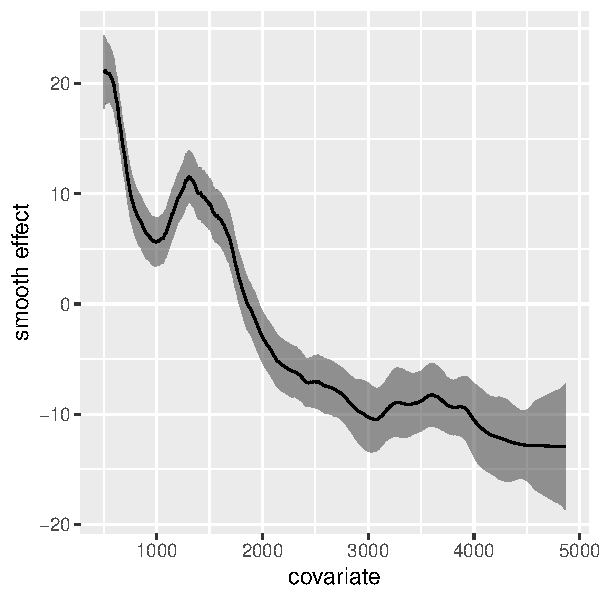
\includegraphics[keepaspectratio]{day1_practical_2_files/figure-pdf/unnamed-chunk-40-1.pdf}}
\end{center}

You might want to have a smoother function by placing a RW2 prior.
Unfortunately, this assumes that all the knots are regularly spaced and
some depth values are too close to be used for building the RW2 priors.
For the case, it is possible to use function~\texttt{inla.group()}~to
bin data into groups according to the values of the covariate:

\begin{Shaded}
\begin{Highlighting}[]
\NormalTok{icit}\SpecialCharTok{$}\NormalTok{depth\_grouped }\OtherTok{\textless{}{-}} \FunctionTok{inla.group}\NormalTok{(icit}\SpecialCharTok{$}\NormalTok{SampleDepth,}\AttributeTok{n=}\DecValTok{50}\NormalTok{)}
\end{Highlighting}
\end{Shaded}

\begin{tcolorbox}[enhanced jigsaw, titlerule=0mm, breakable, opacitybacktitle=0.6, rightrule=.15mm, left=2mm, arc=.35mm, toptitle=1mm, coltitle=black, colframe=quarto-callout-warning-color-frame, opacityback=0, colback=white, bottomrule=.15mm, leftrule=.75mm, colbacktitle=quarto-callout-warning-color!10!white, bottomtitle=1mm, title={Task}, toprule=.15mm]

Re-run the global smoother model using a RW2 prior for the depth
smoother and compare your results with the RW1 model.

Take hint

Use the \texttt{depth\_grouped} covariate to define the smoother.

Click here to see the solution

\begin{Shaded}
\begin{Highlighting}[]
\NormalTok{cmp\_rw2 }\OtherTok{=}  \ErrorTok{\textasciitilde{}} \SpecialCharTok{{-}}\DecValTok{1}\SpecialCharTok{+} \FunctionTok{beta\_0}\NormalTok{(}\DecValTok{1}\NormalTok{) }\SpecialCharTok{+} 
  \FunctionTok{smooth\_g}\NormalTok{(depth\_grouped, }\AttributeTok{model =} \StringTok{"rw2"}\NormalTok{) }\SpecialCharTok{+} 
  \FunctionTok{month\_reff}\NormalTok{(Month\_id, }\AttributeTok{model =} \StringTok{"iid"}\NormalTok{) }

\NormalTok{lik }\OtherTok{=}  \FunctionTok{bru\_obs}\NormalTok{(}\AttributeTok{formula =}\NormalTok{ Sources }\SpecialCharTok{\textasciitilde{}}\NormalTok{.,}
               \AttributeTok{family =} \StringTok{"gaussian"}\NormalTok{,}
               \AttributeTok{data =}\NormalTok{ icit)}

\NormalTok{fit\_rw2 }\OtherTok{=} \FunctionTok{bru}\NormalTok{(cmp\_rw2, lik)}

\FunctionTok{data.frame}\NormalTok{(fit\_rw2}\SpecialCharTok{$}\NormalTok{summary.random}\SpecialCharTok{$}\NormalTok{smooth\_g) }\SpecialCharTok{\%\textgreater{}\%} 
  \FunctionTok{ggplot}\NormalTok{() }\SpecialCharTok{+} 
  \FunctionTok{geom\_ribbon}\NormalTok{(}\FunctionTok{aes}\NormalTok{(ID,}\AttributeTok{ymin =}\NormalTok{ X0}\FloatTok{.025}\NormalTok{quant, }\AttributeTok{ymax=}\NormalTok{ X0}\FloatTok{.975}\NormalTok{quant), }\AttributeTok{alpha =} \FloatTok{0.5}\NormalTok{) }\SpecialCharTok{+} 
  \FunctionTok{geom\_line}\NormalTok{(}\FunctionTok{aes}\NormalTok{(ID,mean)) }\SpecialCharTok{+} 
  \FunctionTok{xlab}\NormalTok{(}\StringTok{"covariate"}\NormalTok{) }\SpecialCharTok{+} \FunctionTok{ylab}\NormalTok{(}\StringTok{"Global smooth effect"}\NormalTok{)}
\end{Highlighting}
\end{Shaded}

\begin{center}
\pandocbounded{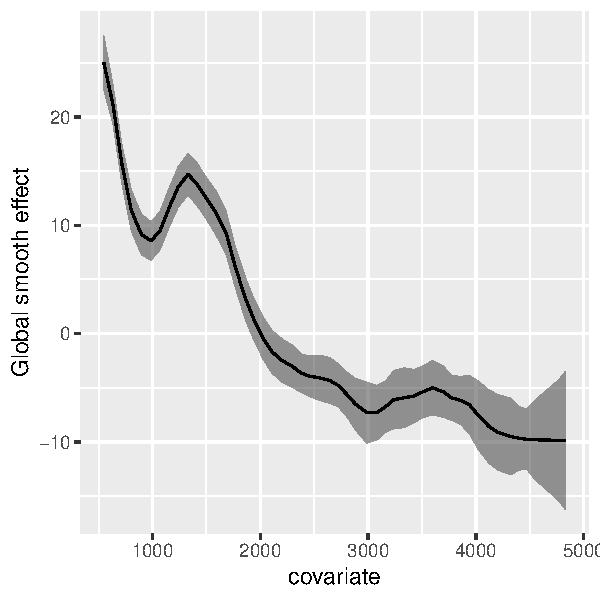
\includegraphics[keepaspectratio]{day1_practical_2_files/figure-pdf/unnamed-chunk-42-1.pdf}}
\end{center}

\end{tcolorbox}

\subsubsection{Fitting group-level
smoothers}\label{fitting-group-level-smoothers}

Here we fit a model where each month is allowed to have its own smoother
for depth, i.e., \(f_i(\text{Depth})_s\). The model structure is given
by:

\[
S_{is} = \beta_0 + f_i(\text{Depth})_s + \text{Month}_i +  \epsilon_{is}.
\]

Notice the only different between the global smoother model (Model G)
and the group level model (Model GS) is the indexing of the smooth
function for depth. We can fit a group-level smoother using the
\texttt{group} argument within the model component as follows:

\begin{Shaded}
\begin{Highlighting}[]
\NormalTok{cmp\_gs }\OtherTok{=}  \ErrorTok{\textasciitilde{}} \SpecialCharTok{{-}}\DecValTok{1}\SpecialCharTok{+} \FunctionTok{beta\_0}\NormalTok{(}\DecValTok{1}\NormalTok{) }\SpecialCharTok{+}
  \FunctionTok{smooth\_g}\NormalTok{(SampleDepth, }\AttributeTok{model =} \StringTok{"rw1"}\NormalTok{) }\SpecialCharTok{+} 
  \FunctionTok{month\_reff}\NormalTok{(Month\_id, }\AttributeTok{model =} \StringTok{"iid"}\NormalTok{)}\SpecialCharTok{+}
  \FunctionTok{smooth\_loc}\NormalTok{(SampleDepth, }\AttributeTok{model =} \StringTok{"rw1"}\NormalTok{, }\AttributeTok{group =}\NormalTok{ Month\_id)}
\end{Highlighting}
\end{Shaded}

Then, we simply run the model (since the observational model has not
changed -only the model components have):

\begin{Shaded}
\begin{Highlighting}[]
\NormalTok{fit\_gs }\OtherTok{=} \FunctionTok{bru}\NormalTok{(cmp\_gs, lik) }
\end{Highlighting}
\end{Shaded}

Lastly, we can generate model predictions using the \texttt{predict}
function.

\begin{Shaded}
\begin{Highlighting}[]
\NormalTok{pred\_gs }\OtherTok{=} \FunctionTok{predict}\NormalTok{(fit\_gs, icit, }\SpecialCharTok{\textasciitilde{}}\NormalTok{ (beta\_0 }\SpecialCharTok{+}\NormalTok{ smooth\_g}\SpecialCharTok{+}\NormalTok{month\_reff}\SpecialCharTok{+}\NormalTok{smooth\_loc))}
\end{Highlighting}
\end{Shaded}

Then, we plot the predicted mean values with their corresponding 95\%
CrIs.

\begin{Shaded}
\begin{Highlighting}[]
\FunctionTok{ggplot}\NormalTok{(pred\_gs,}\FunctionTok{aes}\NormalTok{(}\AttributeTok{y=}\NormalTok{mean,}\AttributeTok{x=}\NormalTok{SampleDepth))}\SpecialCharTok{+}
  \FunctionTok{geom\_ribbon}\NormalTok{(}\FunctionTok{aes}\NormalTok{(SampleDepth,}\AttributeTok{ymin =}\NormalTok{ q0}\FloatTok{.025}\NormalTok{, }\AttributeTok{ymax=}\NormalTok{ q0}\FloatTok{.975}\NormalTok{), }\AttributeTok{alpha =} \FloatTok{0.5}\NormalTok{,}\AttributeTok{fill=}\StringTok{"tomato"}\NormalTok{) }\SpecialCharTok{+}
  \FunctionTok{geom\_line}\NormalTok{()}\SpecialCharTok{+}
  \FunctionTok{geom\_point}\NormalTok{(}\FunctionTok{aes}\NormalTok{(}\AttributeTok{x=}\NormalTok{SampleDepth,}\AttributeTok{y=}\NormalTok{Sources ),}\AttributeTok{alpha=}\FloatTok{0.25}\NormalTok{,}\AttributeTok{col=}\StringTok{"grey40"}\NormalTok{)}\SpecialCharTok{+}
  \FunctionTok{facet\_wrap}\NormalTok{(}\SpecialCharTok{\textasciitilde{}}\NormalTok{Month)}
\end{Highlighting}
\end{Shaded}

\pandocbounded{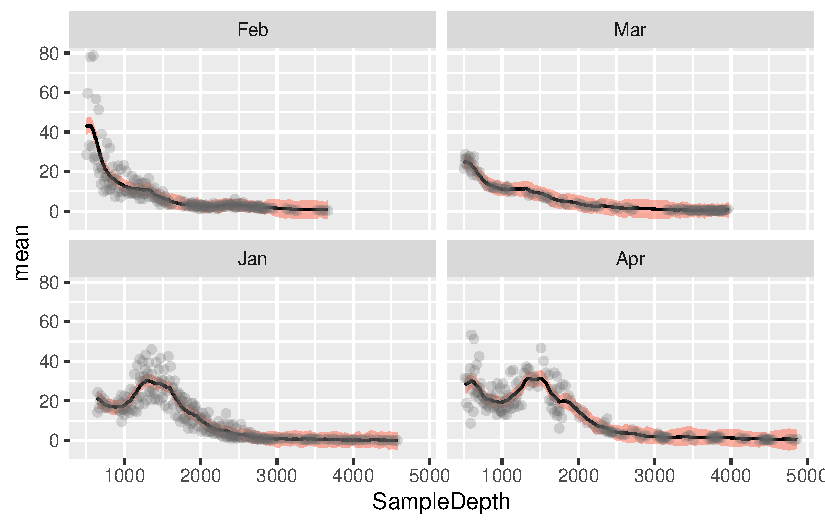
\includegraphics[keepaspectratio]{day1_practical_2_files/figure-pdf/unnamed-chunk-46-1.pdf}}

\begin{tcolorbox}[enhanced jigsaw, titlerule=0mm, breakable, opacitybacktitle=0.6, rightrule=.15mm, left=2mm, arc=.35mm, toptitle=1mm, coltitle=black, colframe=quarto-callout-warning-color-frame, opacityback=0, colback=white, bottomrule=.15mm, leftrule=.75mm, colbacktitle=quarto-callout-warning-color!10!white, bottomtitle=1mm, title={Task}, toprule=.15mm]

Re-fit the model GS without the global smoother. By omitting the global
smoother, we do not longer force group-level smooths to follow a shared
pattern, which is useful when groups may differ substantially from a
common trend.

Take hint

You only need to modify the model components in \texttt{cmp\_gs}

Add hint details here\ldots{}

Click here to see the solution

\begin{Shaded}
\begin{Highlighting}[]
\NormalTok{cmp\_s }\OtherTok{=}  \ErrorTok{\textasciitilde{}} \SpecialCharTok{{-}}\DecValTok{1}\SpecialCharTok{+} \FunctionTok{beta\_0}\NormalTok{(}\DecValTok{1}\NormalTok{) }\SpecialCharTok{+}
  \FunctionTok{month\_reff}\NormalTok{(Month\_id, }\AttributeTok{model =} \StringTok{"iid"}\NormalTok{)}\SpecialCharTok{+}
  \FunctionTok{smooth\_loc}\NormalTok{(SampleDepth, }\AttributeTok{model =} \StringTok{"rw1"}\NormalTok{, }\AttributeTok{group =}\NormalTok{ Month\_id)}

\NormalTok{fit\_s }\OtherTok{=} \FunctionTok{bru}\NormalTok{(cmp\_s, lik) }

\NormalTok{pred\_s }\OtherTok{=} \FunctionTok{predict}\NormalTok{(fit\_s, icit, }\SpecialCharTok{\textasciitilde{}}\NormalTok{ (beta\_0 }\SpecialCharTok{+}\NormalTok{month\_reff}\SpecialCharTok{+}\NormalTok{smooth\_loc))}

\FunctionTok{ggplot}\NormalTok{(pred\_s,}\FunctionTok{aes}\NormalTok{(}\AttributeTok{y=}\NormalTok{mean,}\AttributeTok{x=}\NormalTok{SampleDepth))}\SpecialCharTok{+}
  \FunctionTok{geom\_ribbon}\NormalTok{(}\FunctionTok{aes}\NormalTok{(SampleDepth,}\AttributeTok{ymin =}\NormalTok{ q0}\FloatTok{.025}\NormalTok{, }\AttributeTok{ymax=}\NormalTok{ q0}\FloatTok{.975}\NormalTok{), }\AttributeTok{alpha =} \FloatTok{0.5}\NormalTok{,}\AttributeTok{fill=}\StringTok{"tomato"}\NormalTok{) }\SpecialCharTok{+}
  \FunctionTok{geom\_line}\NormalTok{()}\SpecialCharTok{+}
  \FunctionTok{geom\_point}\NormalTok{(}\FunctionTok{aes}\NormalTok{(}\AttributeTok{x=}\NormalTok{SampleDepth,}\AttributeTok{y=}\NormalTok{Sources ),}\AttributeTok{alpha=}\FloatTok{0.25}\NormalTok{,}\AttributeTok{col=}\StringTok{"grey40"}\NormalTok{)}\SpecialCharTok{+}
  \FunctionTok{facet\_wrap}\NormalTok{(}\SpecialCharTok{\textasciitilde{}}\NormalTok{Month)}
\end{Highlighting}
\end{Shaded}

\begin{center}
\pandocbounded{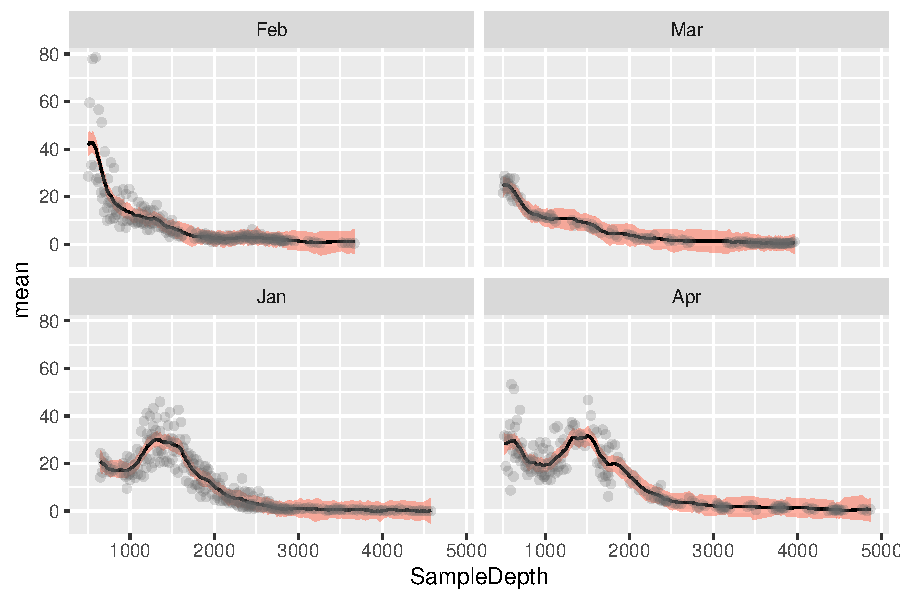
\includegraphics[keepaspectratio]{day1_practical_2_files/figure-pdf/unnamed-chunk-47-1.pdf}}
\end{center}

\end{tcolorbox}




\end{document}
